%%
%% This is file `example-1.tex',
%% generated with the docstrip utility.
%%
%% The original source files were:
%%
%% drexel-thesis.dtx  (with options: `example-part')
%% 
%% This is a generated file.
%% 
%% Copyright (C) 2010 W. Trevor King
%% 
%% This file may be distributed and/or modified under the conditions of
%% the LaTeX Project Public License, either version 1.3 of this license
%% or (at your option) any later version.  The latest version of this
%% license is in:
%% 
%%    http://www.latex-project.org/lppl.txt
%% 
%% and version 1.3 or later is part of all distributions of LaTeX version
%% 2003/06/01 or later.
%% 

\chapter{Quasi 1-D Minicolumns}
Traveling waves in one-dimensional neuronal systems have been previously explored using several theoretical methods.
In the literature on neural fields \citep{Ermentrout1979}\citep{Folias2012} and coupled oscillators \citep{Kopell1986}\citep{Williams1997} isotropic networks of homogeneous neurons with symmetric synaptic coupling give rise to field models which exhibit traveling wave solutions for certain parameter values. 
One-dimensional waves have also been observed in simulations using firing rate neurons \citep{Roxin2005}, integrate-and-fire neurons \citep{Bressloff1997}\citep{Golomb1999} and Hodgkin-Huxley neurons \citep{Golomb1997}.
\citet{Senk2020} used populations of both rate neurons and integrate-and-fire neurons and developed a method to translate parameters between the two different models.
These simulations again use homogeneous neuronal populations in networks that are invariant to spatial translation, resulting naturally in periodic spatio-temporal patterns.
These purely one-dimensional systems may not be robust to realistic variation in neuron properties, connectivity and noise.
This is exemplified in \citet{Senk2020} where traveling waves are only observed for certain parameter values, and \citet{Strogatz1991} where the stability of systems of coupled oscillators can be radically altered by including infinitesimal noise.
Our current work explores traveling waves in quasi-one-dimensional networks with substantial randomness in both individual neurons (randomly selecting type and randomizing dynamical parameters), connectivity between neurons, and stimulus to the neurons.

Previous studies have used one-dimensional structures largely for their computational or analytic simplicity. 
Consideration of a quasi one-dimensional system may seem as an unnecessary complication, but there is no a priori reason that quasi one-dimensional traveling waves may not be found in vivo.
Of interest, there are regions of the brain where there are what seem to be quasi  one-dimensional structures \citep{buxhoeveden2002}\citep{mountcastle1997} typically called micro- or minicolumns. 
These minicolumns are aligned perpendicular to the pia and can be hundreds of microns long.  
Although their relevance to cognition and function is still being debated \citep{horton2005}\citep{Cruz2009}\citep{buxhoeveden2002}, it is possible that they can sustain traveling waves.

To address this possibility, here we investigate the conditions under which traveling waves can exist on quasi one-dimensional systems, and their fundamental properties and dynamics.  
Inspired by minicolumns, our systems consist of thin (few neuron) and long (~100 neuron) networks of locally connected neurons placed on a three-dimensional lattice.  
We model the neuron dynamics using the Izhikevich model \citep{izhikevich2003} that allow us to explore more complex neuron dynamics than typically afforded by integrate-and-fire models \citep{keane2015}\citep{Senk2020} while also providing a distribution of neuron dynamical parameters that mimics the type and variety of neurons observed in the mammalian cortex.
We use a morphology and connectivity model inspired by \citet{maass2002},incorporating a local connectivity model \citep{Levy2012}\citep{Pyle2017}\citep{Fino2011}.
To incorporate elements of a real brain, we consider a model with substantial randomness in both individual neurons and connections between neurons while also considering  distance-dependent time delays in the propagation of action potentials.

Among our main findings we determine parameters in our model that allow for the generation of traveling waves in our quasi one-dimensional systems. 
These traveling waves exhibit properties such as spontaneous creation from a random background stimulus, annihilation of colliding waves, and a wave velocity that is determined by both the propagation speed of the action potential and the neuron dynamics.
Traveling waves are present in both locally-connected and fully-connected systems. 
The traveling waves in fully connected systems are dependent upon the action potential propagation speed, while traveling waves can propagate in locally-connected systems even when action potential propagation is instantaneous.

The results are organized as a series of computational experiments on traveling waves.
We first determine which parameterizations of our model support traveling waves.
Stronger and more numerous local connections between neurons are found to facilitate the formation of traveling wave patters.
We then investigate the influence of neuron dynamics and connectivity on the speed of traveling waves.
Stronger neuronal connections and faster action potential propagation are shown to increase traveling wave speed, but the neuron dynamics enforce an upper limit on the speed. 
Low-threshold-spiking inhibitory neurons are shown to consistently generate traveling waves through the mechanism of post-inhibitory rebound spiking.
The low-threshold-spiking inhibitory neurons also suppress traveling waves that originate from other points in the SCE.
Finally, we examine fully-connected networks and observe that traveling wave patterns can still emerge provided the action potential propagation speed is slow enough.

\section{Minicolumn structure}
We use open boundary conditions, so neurons near the ends of the SCE will have fewer connections than those in the middle.
An example of an SCE showing the connectivity structure is shown in Figure \ref{fig:column_structure}.
\begin{figure}[!htb]
 \caption{Example SCE with dimensions 2x2x10 (XxYxZ), $\lambda$=2.5, and C=1. A)  SCE showing connections between neurons as lines colored using a color scale that indicates the connection length. 
 B)  Connection matrix. E-E connections are green, E-I are black and both I-E and I-I  are red. 
 The labels of the neurons used in both axes are sequentially assigned starting at the bottom (Z=0).
 C) The sum of presynaptic weights for each neuron shows the anisotropy of this model, with substantial variation in input strength and sign between the neuron inputs.}
 \label{fig:column_structure}
 \subfloat[][]{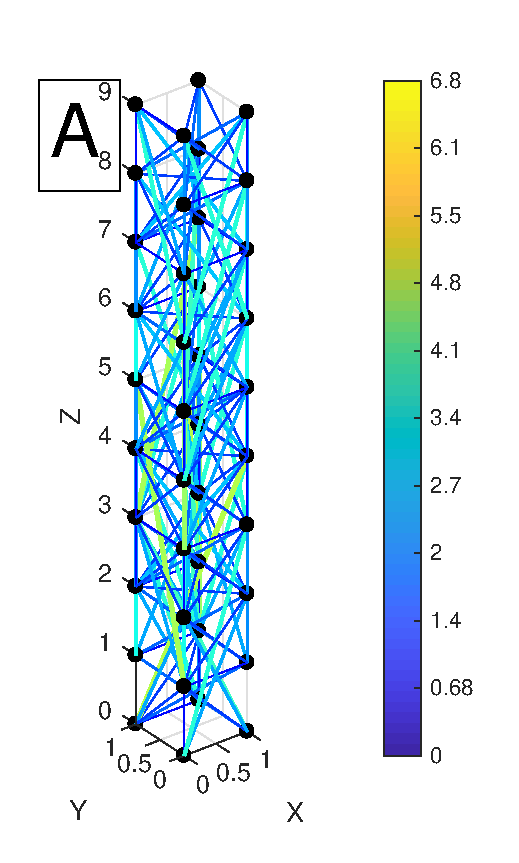
\includegraphics[height=60mm]{fig/column_structure_A}}
 \subfloat[][]{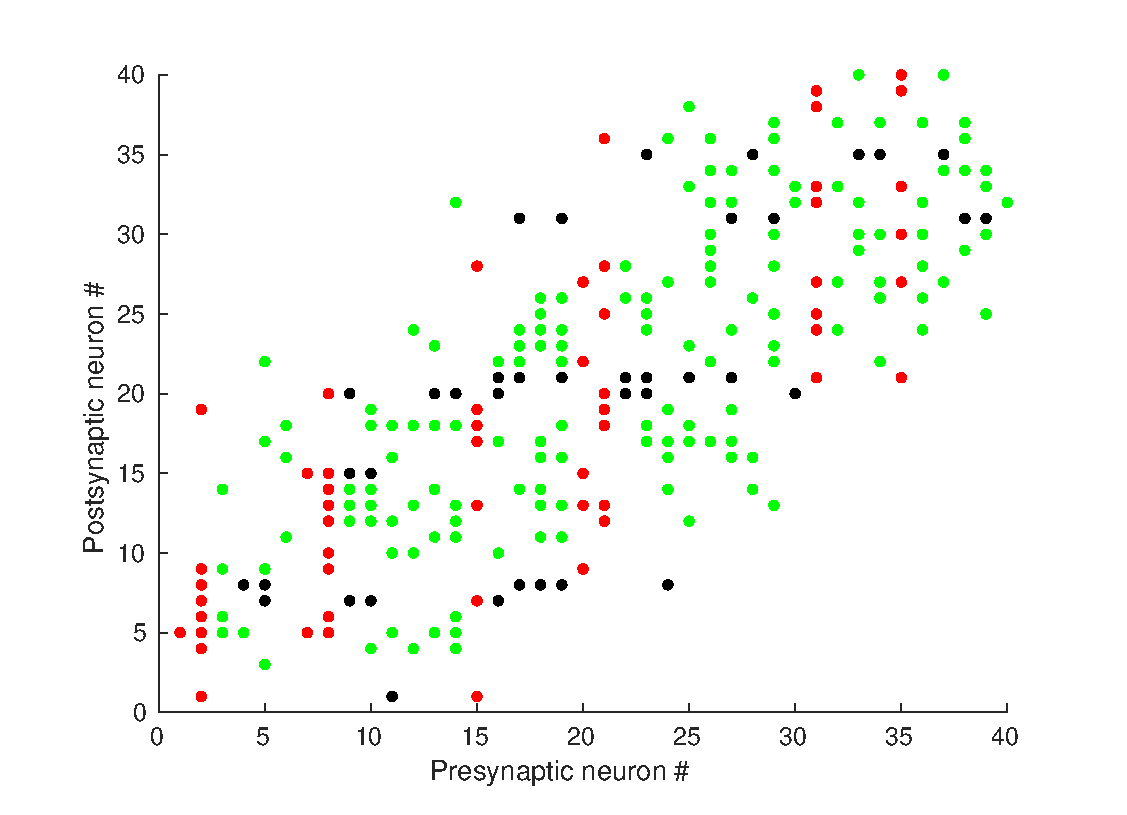
\includegraphics[height=60mm]{fig/column_structure_B}}
 \subfloat[][]{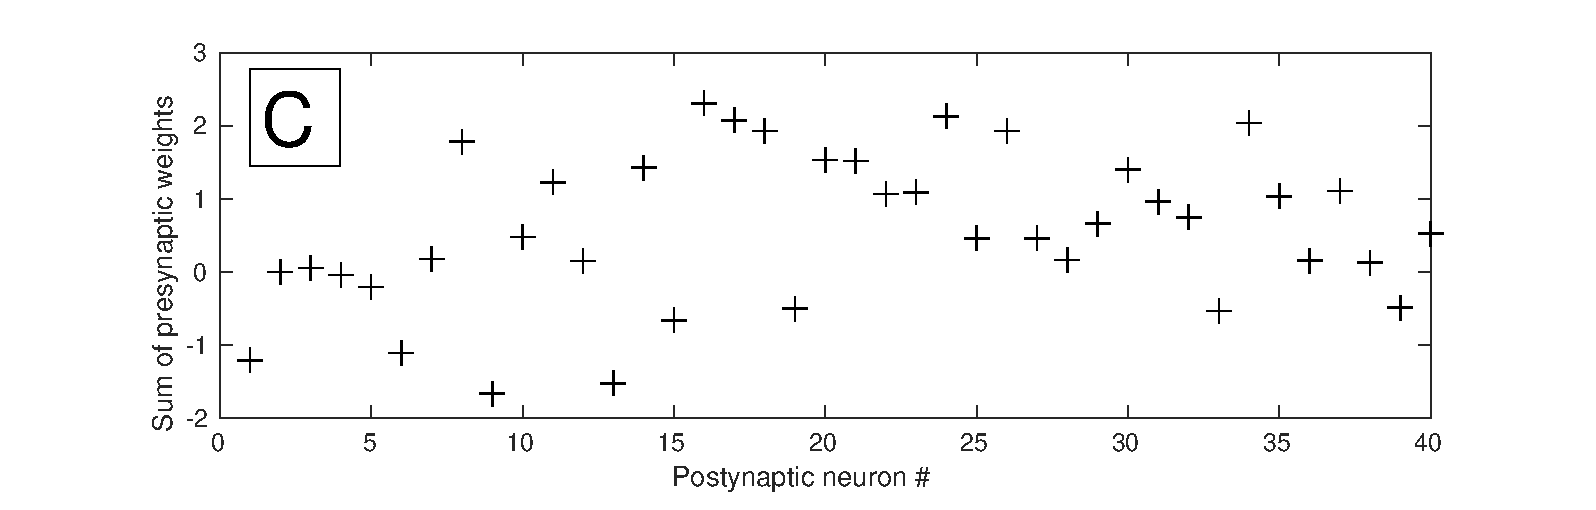
\includegraphics[width=\textwidth]{fig/column_structure_C}}
\end{figure}

A crucial element in neuronal systems is the existence of time delays between the creation of a presynaptic action potential and the arrival of that spike to a target neuron. 
We use distance-dependent time delays for the propagation of a spike from neuron $i$ to neuron $j$ of $\tau_{ij} = \kappa  D(i,j)$. 
The constant of proportionality $\kappa$ ranges from $0$ to $4$.
When $\kappa=0$ the action potential excites the post-synaptic neuron on the succeeding simulation time step.
 
The distribution of post-synaptic connections and delay times are shown in Figure \ref{fig:connection_delay_distrbution} for an example minicolumn.
\begin{figure}[!htb]
 \caption{Distribution of (A) number of post-synaptic connections per neuron and (B) delay time. Data was taken over 100 realizations of a 2x2x50 SCE, $\lambda=2.5$, $\kappa=1$.  } 
 \begin{tabular}{c}
     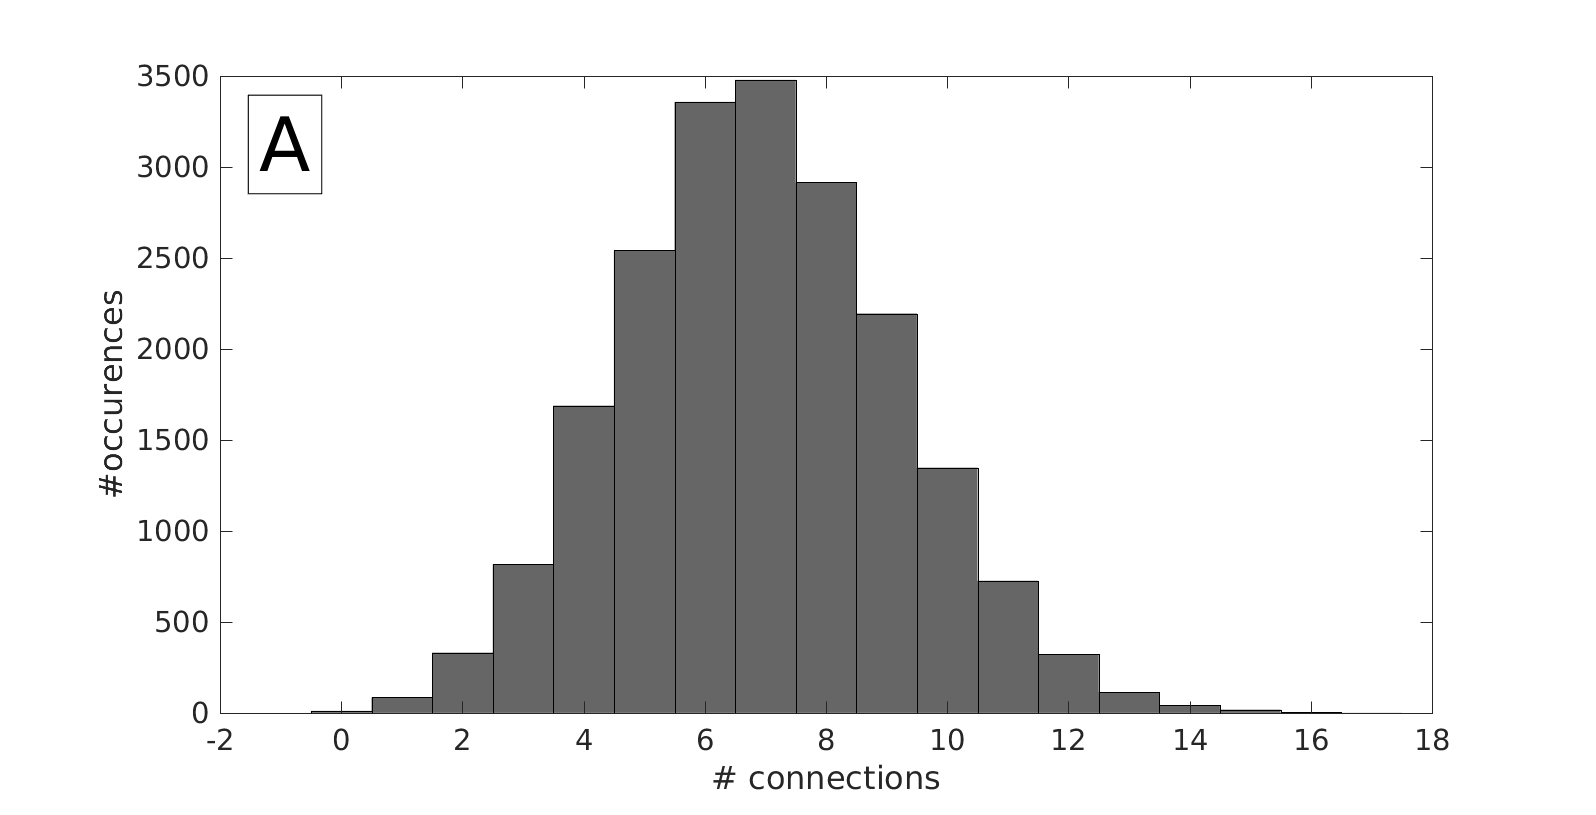
\includegraphics[width=\textwidth]{fig/ConnectionNumberDistribution} \\
     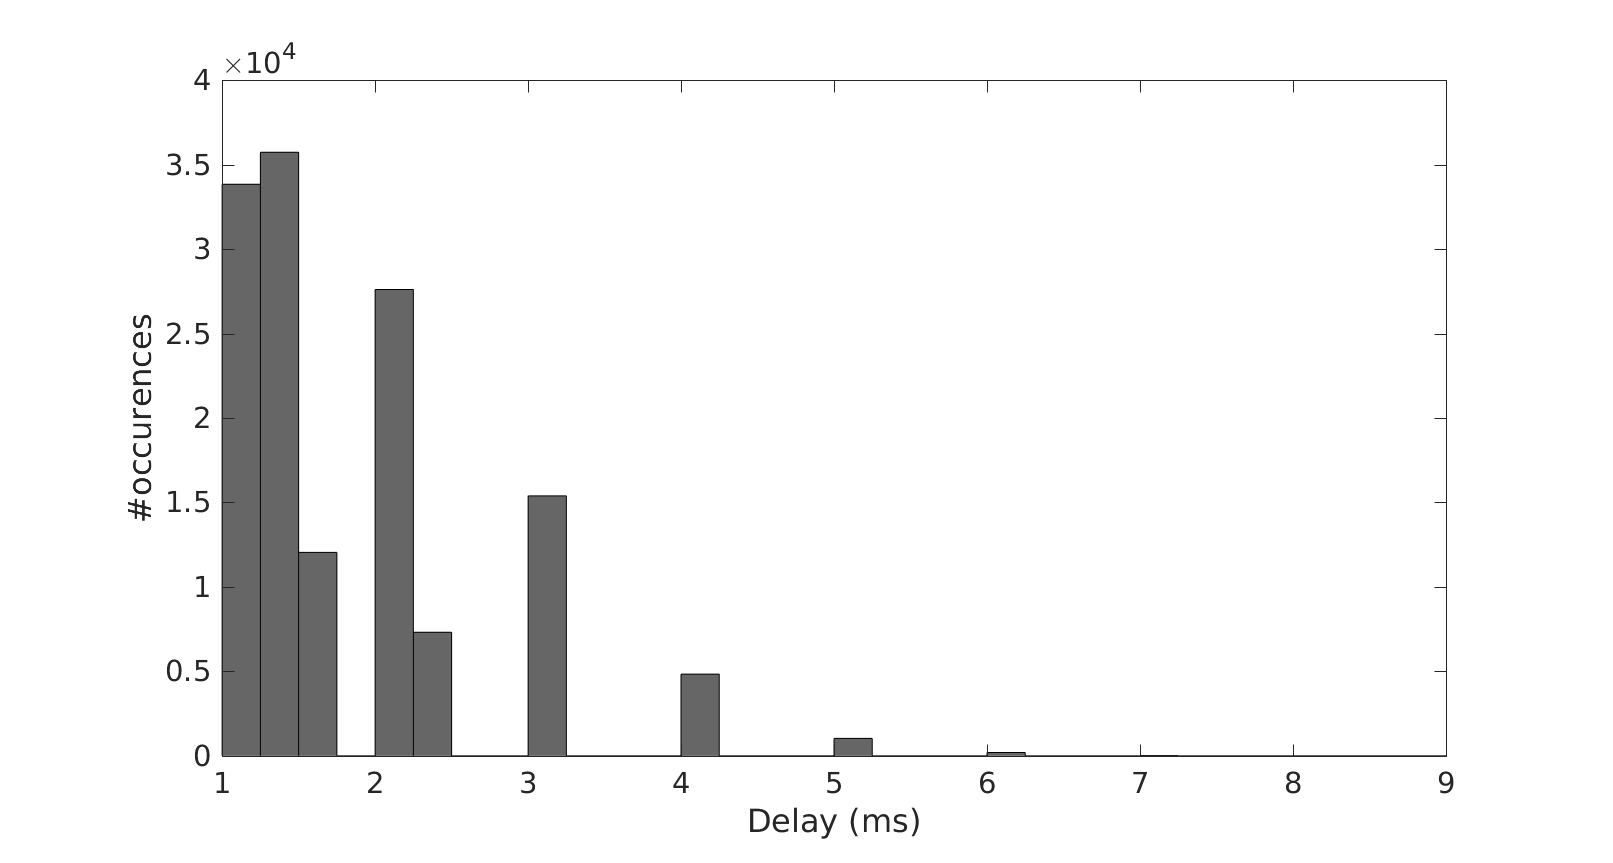
\includegraphics[width=\textwidth]{fig/DelayDistribution} 
 \end{tabular}
 \label{fig:connection_delay_distrbution}
\end{figure}
 \FloatBarrier
 
For every simulation we record all of the spikes from all neurons. 
We visualize the spikes in spike raster plots (e.g. Figure \ref{fig:sigma_raster} ).
Because here we focus on traveling waves in the Z direction, we plot the spikes according to the Z position of the neurons.
As a consequence, at each Z position there are multiple neurons that could contribute to the spike raster plot at that Z coordinate (e.g. 4 neurons for the X=2, Y=2 SCE case).

To automatically identify waves we perform a spatial clustering operation to this data to identify spatiotemporal regions identified by high firing density. 
The clustering operation produces an output cluster for any group of more than $3$ spike events that fall within a $20ms$ time window from neurons that are no more than $3$ layers apart.
Each cluster $C(t,z)$ has a time $t$ and position $z$.
This clustering removes random background firing activity. 
The waves are identified using a plane sweep algorithm that proceeds along the dimension of simulation time and applies wave labels to clusters such that all clusters with the same label are part of the same wave.
When a new cluster $C(t,z)$ is encountered, the algorithm associates $C(t,z)$ with any existing wave if the existing wave has a cluster $C(t_c,z_c)$ within $40 ms$ and $6$ units of the new cluster.
If there is no such adjacent cluster a new wave is created using $C(t,z)$ as the first cluster.

An example of the clustering and identification is shown in Figure 2, with further illustration in SI Figure 1.
\begin{figure}[!htb]
 \centering
 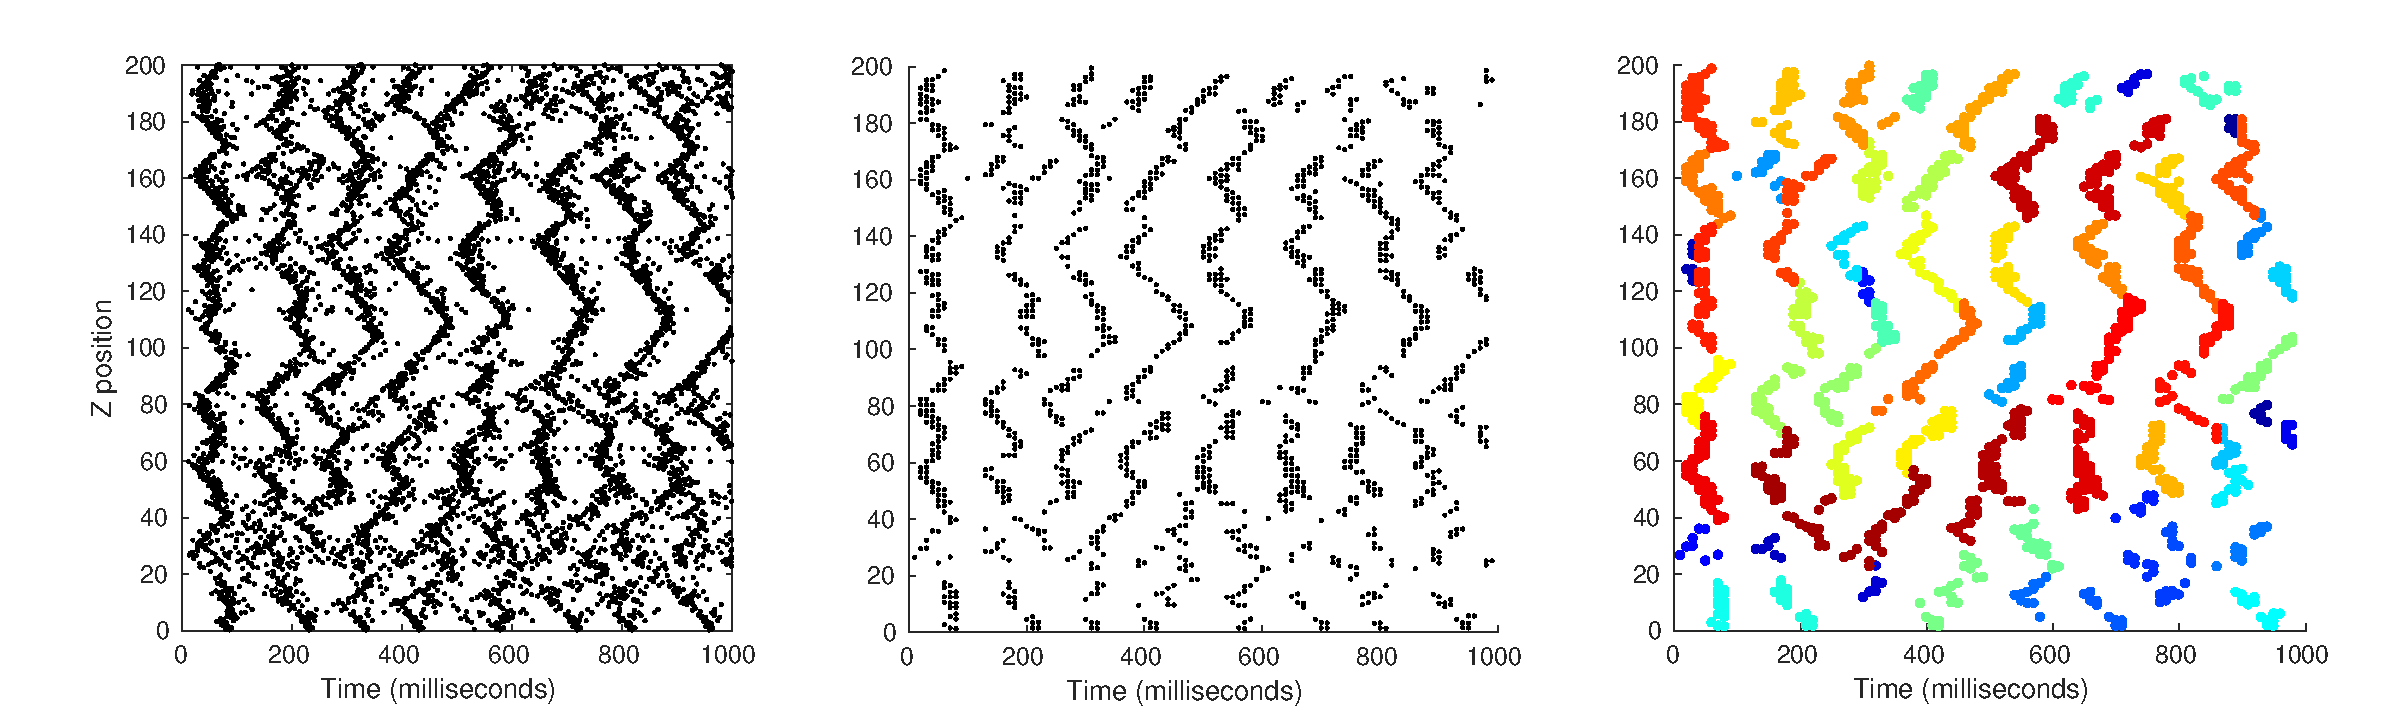
\includegraphics[width=\textwidth]{fig/DetectorExample}
 \caption{Wave identification and labeling using an example SCE with dimensions 2x2x200 . Left: Raster plot of firing events where dots represent neuronal action potentials. 
          Traveling waves can be seen as diagonal structures of dense firing activity. 
          Center: The clustering operation removes background spikes. 
          Right: Individual waves are labeled with unique identifiers color coded in the figure.}
 \label{fig:wave_analysis}
\end{figure}

Our wave detection and analysis approach must remain valid across a range of model parameters. 
We show sample visualizations for varying values of $K$ in Figure \ref{fig:detector_test}.
This detector test demonstrates that our detection and analysis method detects and labels traveling waves of various lengths even in a noisy background.
\begin{figure}[!htb]
 \caption{The clustering and wave labeling process. Spike raster plot (left), filtered clusters (middle) and labeled waves (right, each color is a unique wave) are shown for SCE with different values of $K$. }
 \label{fig:detector_test}
 \centering
   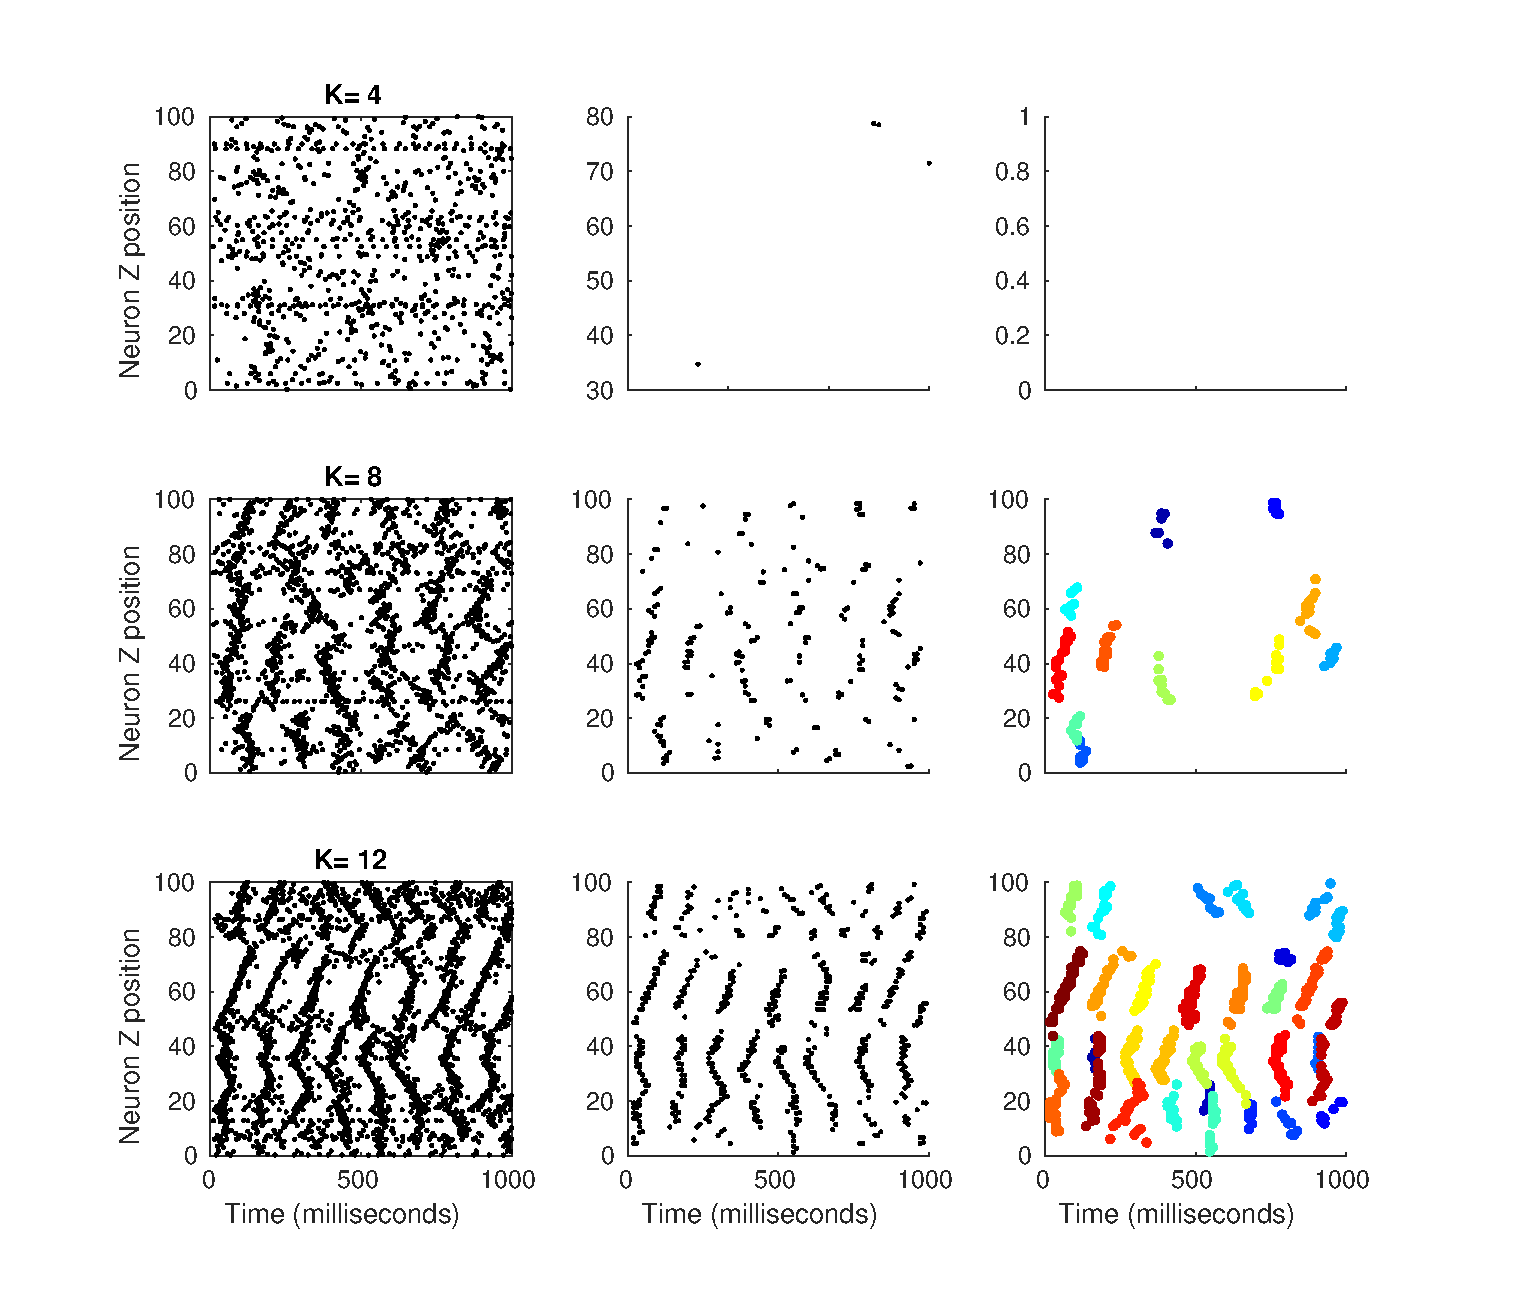
\includegraphics[width=\textwidth]{fig/DetectorTest}
\end{figure}

\FloatBarrier
Once identified and labeled, we measure wave propagation speeds and wave initiation locations. 
We also measure the "wave firing fraction" defined as the fraction of spikes that are associated with the labeled traveling wave (total number of spikes found within the waves divided by number of spikes in the simulation). 

Our exploration of the behavior of traveling waves in an SCE involves testing properties of these waves as a function of the different parameters of our model.
For determining existence of traveling waves we use a $2x2x100$ SCE  with background stimulation (Eq \ref{eq:randomstim}) and vary parameters around a neighborhood of the reference point $\Sigma = \{K=10,\lambda=2.5,P_{exc}=0.8,\kappa=1.0 \}$ that we have determined can sustain traveling waves.
To measure wave propagation speed we use a $2x2x50$ SCE with  a step stimulus applied to the lowest layers of the SCE and adjust our reference point to be $\Sigma_v = \{K=24,\lambda=2.5,P_{exc}=0.8,\kappa=1.0 \}$.
This reference point was selected after inspecting the SCE behavior under a wide range of parameter values.
The increase in $K$ is required when using the step stimulus because the higher layers of the SCE do not receive any stimulus.
This requires stronger connections so that the traveling wave can elicit spikes from neurons resting at equilibrium.

\FloatBarrier

\section{Existence of 1-D waves} \label{sub:waves}
We first explore which parameterizations of our model will support traveling waves.
We detect the waves as described in Methods, and then use the wave firing fraction metric to determine for which parameter values our model will produce traveling waves.
We fix the connection normalization constant $C$ in equation \ref{eq:connectivity} to $0.5$ and we fix the stimulus strength $M$ in equation \ref{eq:randomstim} to $5$.
For this value of C and $\lambda=2.5$ each neuron has an average of $6.90$ input connections, as measured across $100$ randomly-generated SCE (see SI Figure 2 for connectivity distribution).

The key parameters of our model that we examine are the connection strength $K$, the characteristic connection length $\lambda$, the fraction of excitatory neurons $P_{exc}$ and the delay parameter $\kappa$.
First we establish that traveling waves are observed at the reference  point $\Sigma = \{K=10,\lambda=2.5,P_{exc}=0.8,\kappa=1.0 \}$.
We then vary the individual parameters about $\Sigma$ to examine how they influence traveling wave formation.

At the reference  point $\Sigma$ the average wave firing fraction over 100 trials is found to be $88.6\%$ with a standard deviation of $4.38\%$.
A representative raster plot of the spike events (Figure \ref{fig:sigma_raster}) clearly shows the traveling waves.
\begin{figure}[!htb]
 \centering
 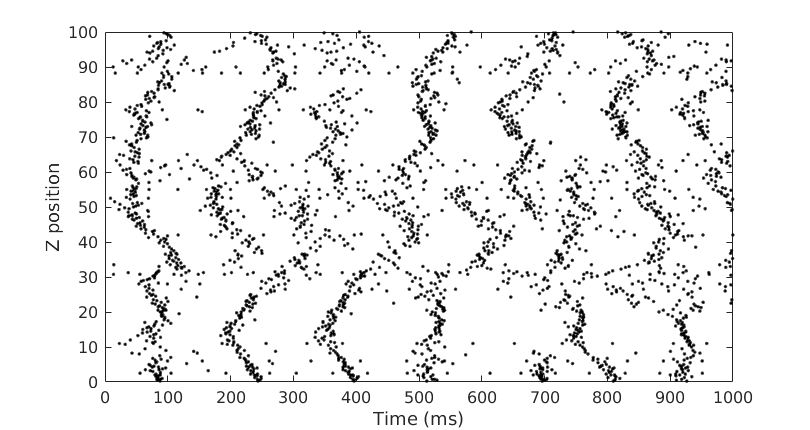
\includegraphics[width=0.75\textwidth]{fig/baseline}
 \caption{Raster plot of neuron firing events over time. The model parameters are at the reference  point $\Sigma$. Each dot represents the spike-time emission of a neuron. Traveling waves can be seen as diagonal structures of dense firing activity \citet{Senk2020}. }
 \label{fig:sigma_raster}
\end{figure}

The effect of varying the parameters on traveling waves are shown in Figure \ref{fig:wave_parameters}.
The graphs of the wave firing fraction versus $K$, $\lambda$ and $P_{exc}$ show similar behavior.
Traveling waves are not supported for low values of these parameters.
As the parameter values increase traveling waves emerge, and as the parameters grow large the traveling waves dominate the firing activity.
Stronger connections ($K$) or more numerous connections ($\lambda$) makes it easier for firing activity to spread to adjacent neurons.
A higher excitatory fraction acts similarly to a higher connection strength. 
As the presynaptic activity to each neuron is more excitatory and less inhibitory, it is easier for the traveling wave to propagate.
These data suggest that these three parameters all work towards strengthening the local neighborhood of neurons and facilitating the propagation of coordinated spikes as traveling waves.

\begin{figure}[!htb]
 \centering
 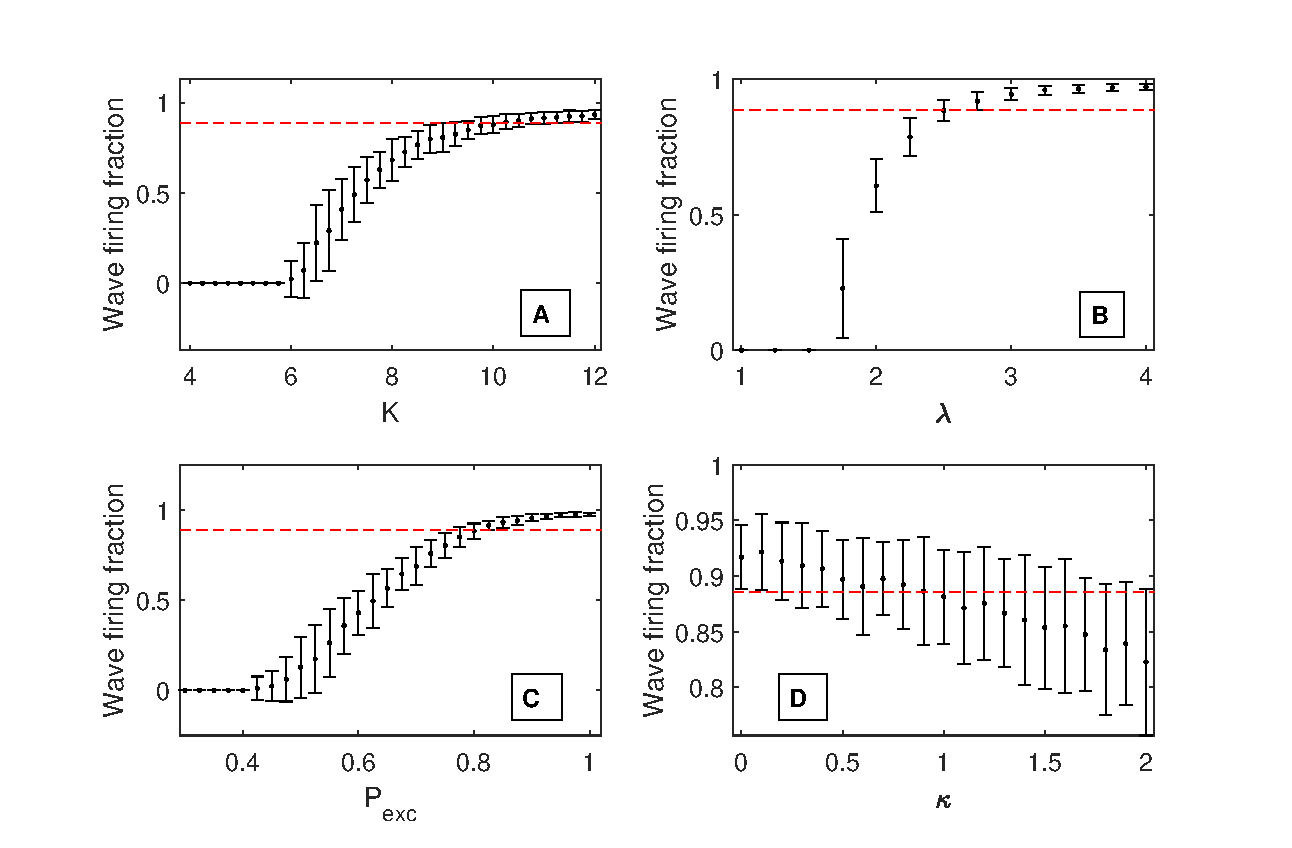
\includegraphics[width=\textwidth]{fig/ParamWaveSim}
 \caption{Onset of traveling waves as a function of model parameters in the neighborhood of $\Sigma$ (100 trials for each parameter value, error bars $1\sigma$). 
         The dashed red lines show the wave firing fraction at the reference  point $\Sigma$.  
         Varying each individual parameter while holding the other parameters at their $\Sigma$ values, we observe onset of traveling waves at $K=6$ (A), $\lambda=1.5$ (B), and $P_{exc}=0.45$ (C).  
         D) Traveling waves are present at all values of $\kappa$. }
 \label{fig:wave_parameters}
\end{figure}

\FloatBarrier

For the range of values tested, the parameter $\kappa$ does not show a strong influence on the existence of traveling waves. 
This is in contrast to previous work in largely isotropic networks and neural field models which found that the delay parameter is important for the emergence of traveling waves \citet{Senk2020}\citet{Atay2006}\citet{Roxin2005}.
However, it is consistent with other work that found traveling wave patterns without including propagation delay \citet{Folias2012}\citet{Wyller2007}.

A natural question is whether the few long connections along the Z direction that cannot exist in the X or Y directions exert a dominant role on these results.
By performing the same experiments as in Figure 4, but now pruning long-range connections, results show that the influence of the longer connections is minimal (SI Figure 4).

We establish purely one-dimensional systems in our model for comparison to previous work with purely one-dimensional systems.
We start with the SCE described in Section 3.1 for measuring wave speed: a 2x2x50 (XxYxZ) SCE with model parameters at the reference point $\Sigma_v$. 
While previous work with this SCE measured the speed of the waves, here we determine the existence of traveling waves based on whether the neurons in the top layer of the SCE fire.
\textbf{The baseline quasi one-dimensional SCE creates 74 traveling waves in 100 trials}, where each trial is a random draw on all randomized parameters in the model and stimulus.
An example raster plot is shown in Figure \ref{fig:OneDimensionalRasterPlots}A.

We create a purely one-dimensional version of this SCE with X=1 and Y=1 and all other model parameters at $\Sigma_v$.
\textbf{No traveling waves are observed in this SCE in 100 trials}. 
An example raster plot is shown in Figure \ref{fig:OneDimensionalRasterPlots}B.
We then modify this purely one-dimensional SCE by increasing $\lambda$ from $2.5$ to $4$ and increasing $K$ from $2$4 to $30$.
These parameters represent the highest connectivity and connection strength tested in our quasi one-dimensional SCE.
\textbf{We still do not observe any traveling waves in 100 trials} of this SCE with enhanced connectivity and connection strength.
An example raster plot is shown in Figure \ref{fig:OneDimensionalRasterPlots}C.

Finally we look to remove the random elements of our model to make it more comparable to previous work.
We set $C=1.0$ to create a more uniform and isotropic connectivity between the neurons.
We set $P_{exc}=1$ so that all neurons are excitatory with no inhibitory neurons at random locations.
We remove all random factors from the Izhikevich model parameters a, b, c and d (Table 1).
All neurons therefore have identical dynamics.
\textbf{With this more uniform model we observe 98 traveling waves in 100 trials}, reproducing previous results that have found traveling waves in purely one-dimensional networks.
An example raster plot is shown in Figure \ref{fig:OneDimensionalRasterPlots}D.
Although we have removed most variation from this SCE, the two trials with no waves are not unexpected as the stimulus is still randomized and the connectivity is still probabilistic (see Equation 1).

\begin{figure}[!htb]
 \caption{ Example raster plots of the SCE used for comparison to previous work in purely one-dimensional systems.
           A) The 2x2x50 SCE with model parameters at $\Sigma_v$ supports traveling waves along the entire SCE. 
	   B) The 1x1x50 version of the same SCE does not exhibit traveling waves.
	   C) Even with $K$ increased from $24$ to $30$ and $\lambda$ increased from $2.5$ to $4$, the 1x1x50 SCE still does not support traveling waves.
	   D) Once the random parameters are removed, the 1x1 SCE does support traveling waves. }
   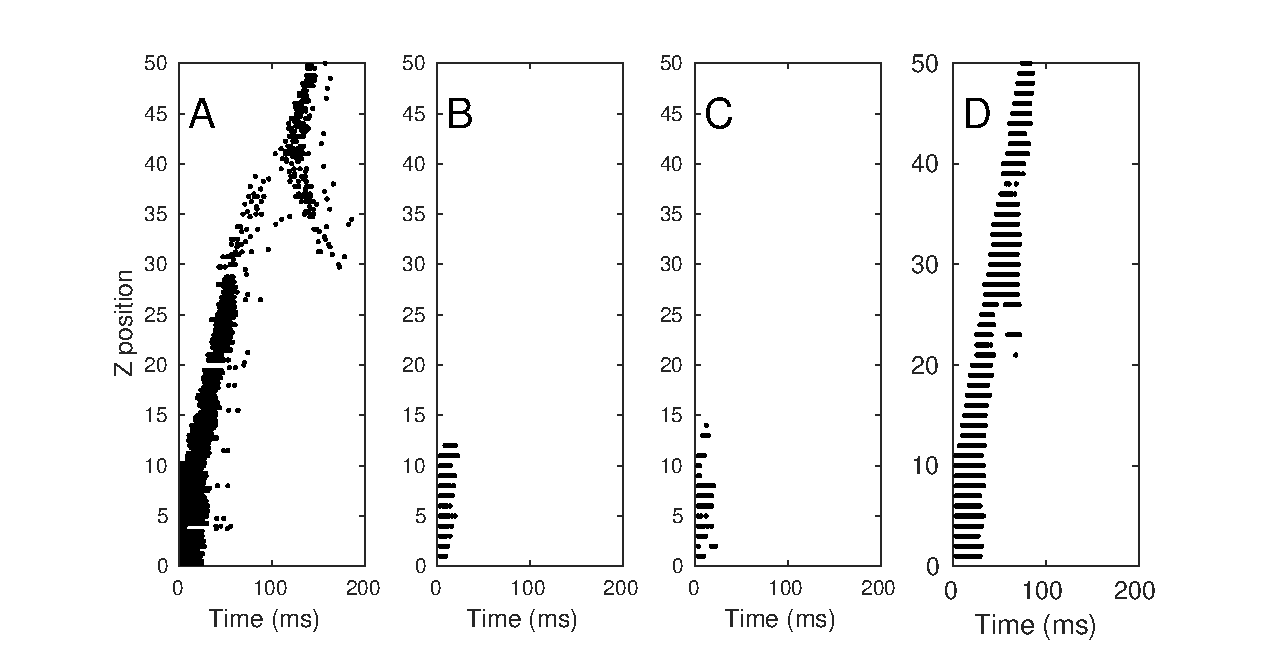
\includegraphics[width=\textwidth]{fig/OneDimensionalComparison_RasterPlots}
   \label{fig:OneDimensionalRasterPlots}
\end{figure}
\FloatBarrier

\section{Wave propagation speed} \label{sub:propagation_speed}
Cortical traveling waves have been observed with propagating speeds from less than $0.1$ to more than $0.8$ meters per second \citet{Sato2012}\citet{Golomb1997}\citet{Chervin1988}.
This is consistent with the action potential propagation speeds in the gray matter of the cortex \citet{Muller2018}. 
This suggests that the dynamics of action potential propagation influence wave propagation. 
To consider the possibility of this relationship we incorporate in our model an action potential propagation time proportional to the distance between the neurons.

Action potential velocity may not be the only factor in the traveling wave propagation speed.
In \citet{Golomb1997} the authors neglected action potential propagation in their model of disinhibited cortical slices as they considered their observed wave velocity of $~0.15 m/s$ to be an order of magnitude faster than axon potential propagation.
In \citet{Chervin1988} the authors found an even slower propagation of $0.06-0.09 m/s$ in disinhibited slices of rat cortex.
In  \citet{Markram1997} a latency of $1.7\pm 0.9\ ms$ was observed between injecting a stimulus in one pyramidal neuron and the resulting excitatory post-synpatic potential in an adjacent pyramidal neuron.
This latency is too large to be due solely to axonal propagation alone given the very short distance between the neurons. 
These results indicate that a second key element, namely neuron and synapse dynamics, will also influence wave propagation speed.
Biological neurons and synapses  have complex internal dynamics, and will not fire instantaneously upon receiving a stimulus.
The input may push the neuron's dynamical system out of equilibrium and cause a spike, but the system dynamics take some time to evolve.
Therefore the spike will occur with some delay after the stimulus.
This is a common behavior in any multidimensional model of neuron dynamics, but it is not captured by the leaky integrate-and-fire model used in much of the previous research \citet{keane2015}\citet{Senk2020}.
As an example, Figure \ref{fig:delay_neuronstep} shows the delayed response of a neuron to a pulse of current using the Izhikevich model.
\begin{figure}[!htb]
 \caption{ A pulse of voltage (bottom) with magnitude $2 mV$, starting at $t=100 ms$ and lasting $2 ms$ disturbs the equilibrium membrane potential of a neuron (top), eliciting a spike at $t=112 ms$. }
 \label{fig:delay_neuronstep}
 \centering
   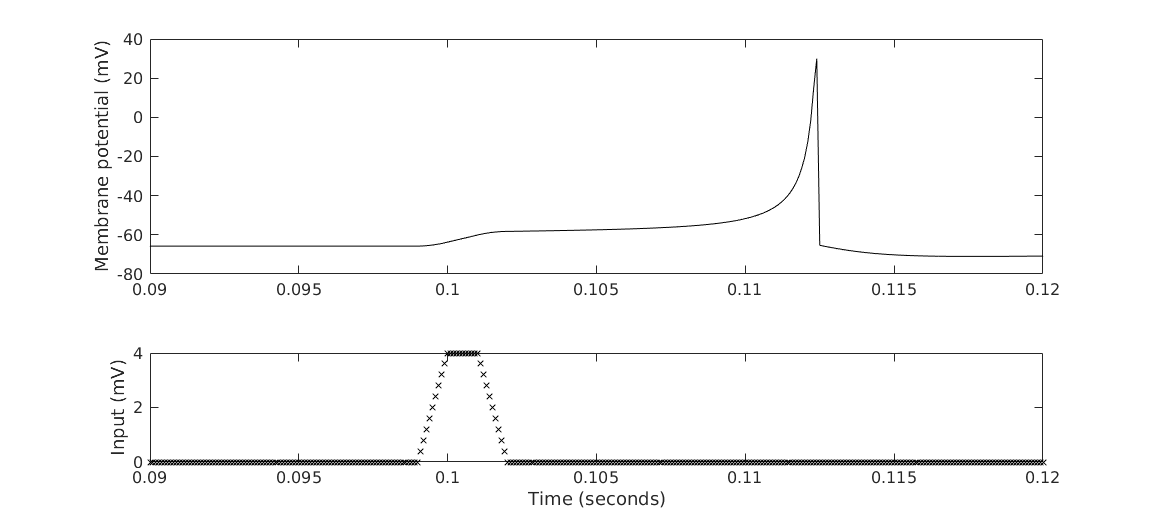
\includegraphics[width=\textwidth]{fig/WaveSpeed_NeuronStepTest}
\end{figure}

To determine  that this spike delay is indeed important to consider  we expose populations of excitatory and inhibitory neurons to current pulses of different magnitudes.
The average firing delay of the excitatory and inhibitory neurons is shown in Figure \ref{fig:delay_neurondynamics}.
The inhibitory neurons have a lower firing threshold than the excitatory neurons due to their higher value of $b$ in Equation \ref{eq:neuron_v}  \citet{izhikevich2003} and fire with a shorter delay when given the same stimulus.
Both excitatory and inhibitory neurons exhibit a delayed response of several $ms$ or more.
\begin{figure}[!htb]
 \caption{ A stronger stimulus creates a spike with less delay. The excitatory neurons have a higher firing threshold than the inhibitory neurons and do not emit a spike for very weak stimulus.}
 \label{fig:delay_neurondynamics}
 \centering
   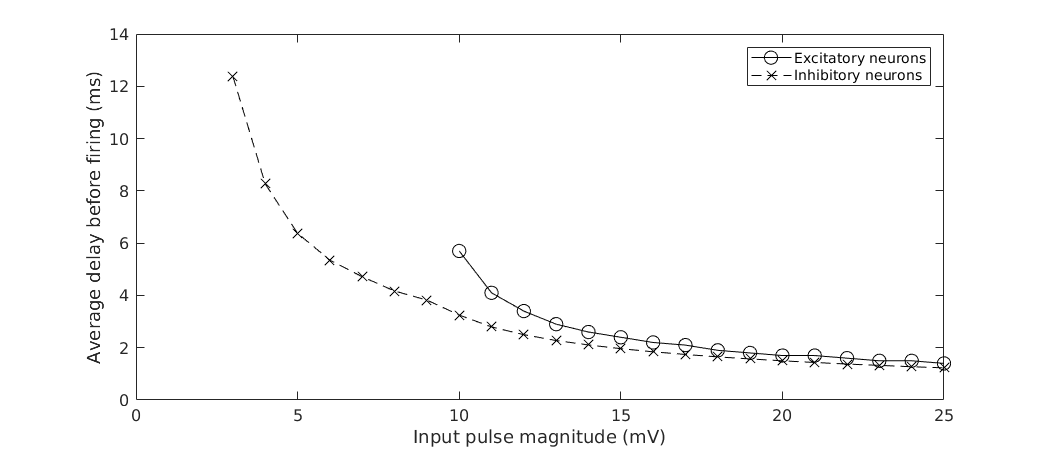
\includegraphics[width=\textwidth]{fig/WaveSpeed_NeuronDynamics}
\end{figure}

\FloatBarrier

To measure wave propagation speed we use an SCE with width 2, height 2, and length 50.
Our exploration of wave speed uses a step stimulus applied to the lowest 10 layers of neurons (see Methods), while no stimulus is applied to the remaining neurons.
We then measure the time for the wave to propagate to the top layer to determine the pace in milliseconds per unit length traveled.
The speed is then calculated as the inverse of the pace in units/millisecond.

We fix the connection normalization constant $C$ in equation \ref{eq:connectivity} to $0.5$ and we fix the stimulus strength $M$ in equation \ref{eq:randomstim} to $5$ and do not vary them.
As mentioned in Methods we use $\Sigma_v$ here, with $K=24$, because the SCE cannot sustain traveling waves at $\Sigma$. 
Here, without the uniform background stimulus the neurons in the SCE are at their equilibrium point when the traveling wave arrives, and it takes a stronger stimulus from the passing wave to elicit a spike.
We increase the connection strength $K$ to provide this stronger stimulus, and find traveling waves that span the SCE starting at $K=18$. 
As $K$ increases the neurons fire with less delay, resulting in faster traveling waves (Figure \ref{fig:delay_k}).
We fix $\Sigma_v = \{K=24,\lambda=2.5,P_{exc}=0.8,\kappa=1.0 \}$ for the remainder of the wave speed computational experiments.

 
We first examine the impact of K on the wave speed.
The wave speed increases with K as anticipated (Figure \ref{fig:delay_k}).
The relationship is logarithmic in shape, in agreement with some previous work including \citet{Golomb1999} (Figure 3 for $\tau_d>0$) and \citet{Golomb1996}(Figure 10, exponential footprint shape).


\begin{figure}[!htb]
 \caption{The pace (left, error bars $\pm 1 \sigma$) decreases with $K$, while the corresponding wave speed (right) increases with $K$. 
          The logarithmic best fit is $0.36\log{0.12K}$.}
 \label{fig:delay_k}
 \centering
   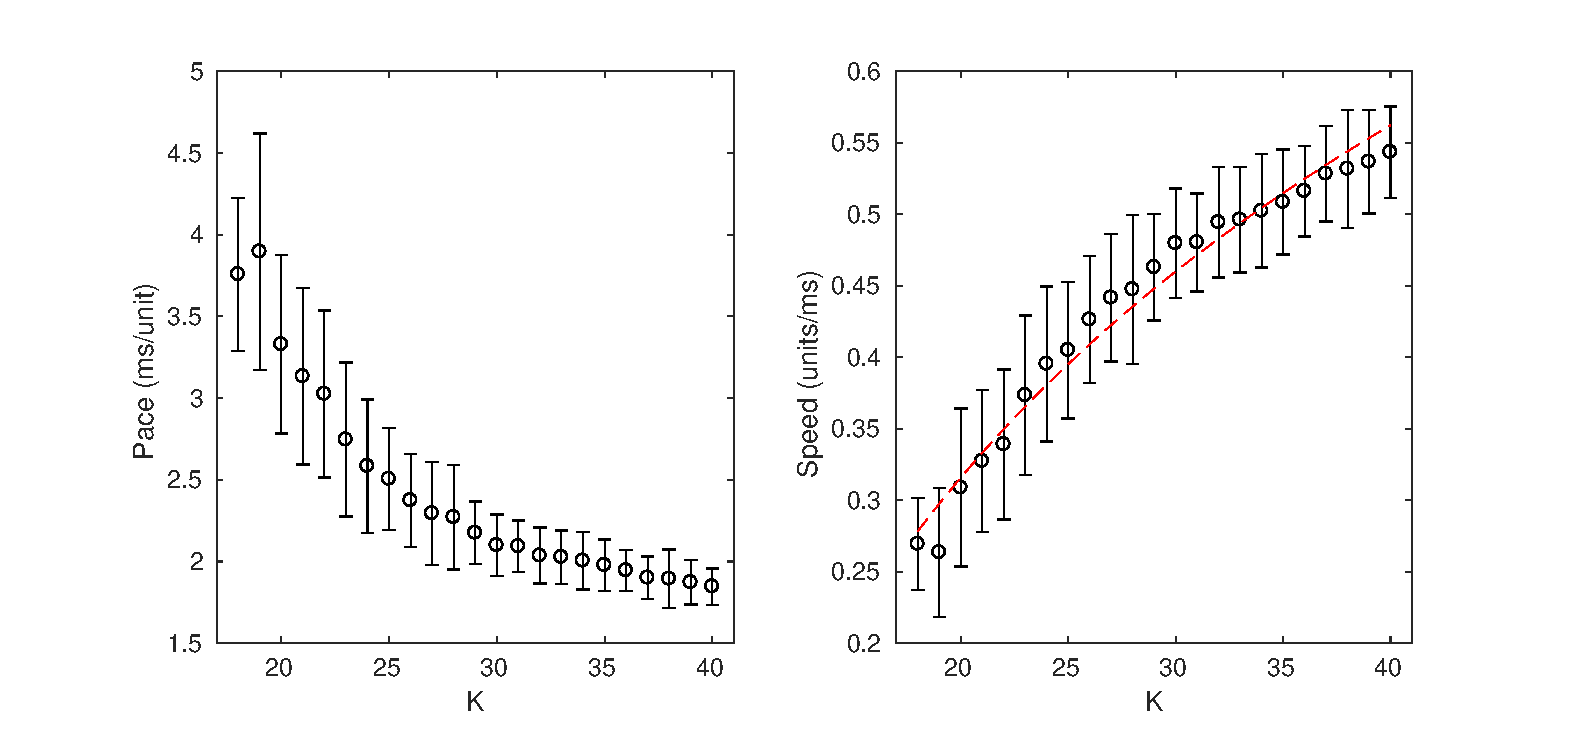
\includegraphics[width=\textwidth]{fig/WaveSpeed_K}
\end{figure}


We examine the influence of the $b$ parameter on wave speed.
We generate $100$ SCE, then multiply the $b$ parameter of all neurons by a scaling factor from $0.7$ to $1.3$.
When the scale factor is $\leq 1.0$ the wave speed remains constant, but when the scale factor is $>1.0$ the wave speed increases linearly (Figure \ref{fig:WaveSpeed_B}).
This indicates that the lower firing thresholds (Figure 6) that result from larger values of the $b$ parameter result in faster traveling waves.

\begin{figure}[!htb]
 \caption{The pace (left, error bars $\pm 1 \sigma$) and the wave speed (right) show a sharp transition above scale factor $1.0$. }
 \label{fig:WaveSpeed_B}
 \centering
   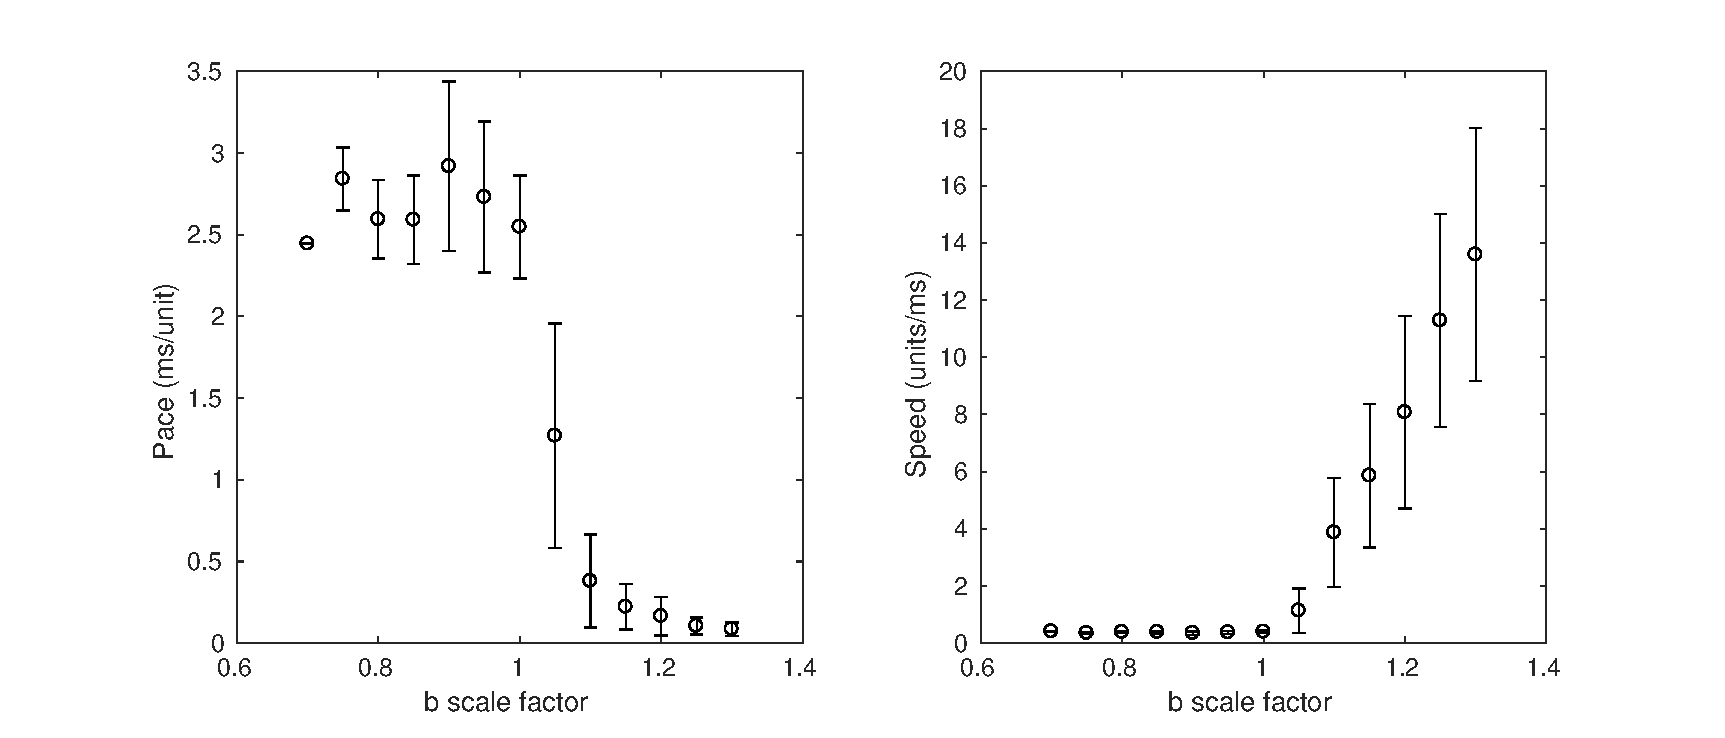
\includegraphics[width=\textwidth]{fig/WaveSpeed_B}
\end{figure}

\FloatBarrier

We next explore the influence of the action potential propagation speed, here controlled by our parameter $\kappa$, on the traveling wave propagation speed.
We vary delay parameter $\kappa$ from 0 to 5 and measure the wave pace and calculate the wave speed (Figure \ref{fig:delay_speed}).
The pace is linear in $\kappa$ as expected, but the pace does not approach $0$ as $\kappa \rightarrow 0$ due to the delayed firing inherent in the neuron dynamics.
Because each neuron does not fire instantaneously upon receiving an action potential, even instantaneous transport of action potentials does not result in a wave that can span the column instantaneously.
\begin{figure}[!htb]
 \caption{The pace (left, error bars $\pm 1 \sigma$) is linear w.r.t. $\kappa$. The intercept at $\kappa=0$ is 1.3, indicating that the neuron dynamics limit the speed of the wave. The wave speed (right) shows the expected relationship. }
 \label{fig:delay_speed}
 \centering
   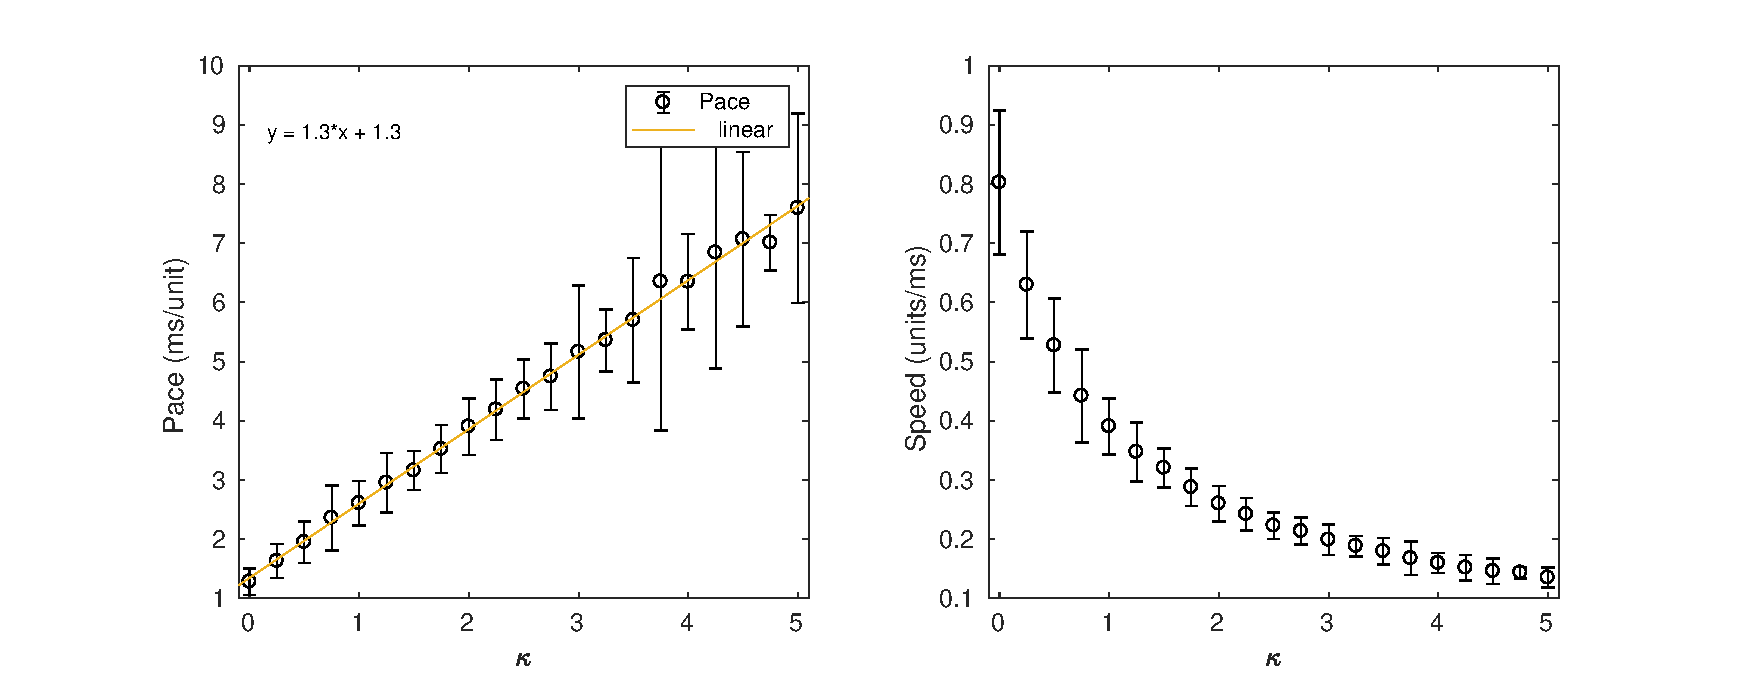
\includegraphics[width=\textwidth]{fig/WaveSpeed_Delay}
\end{figure}
\FloatBarrier

Propagation speed is also influenced by the characteristic length of the local connectivity, $\lambda$.
Since an increase in $\lambda$ results in both longer range connections, and more incoming and outgoing connections per neuron, we expect $\lambda$ to increase the wave speed through both action potential propagation and neuron dynamics.
The characteristic connection length $\lambda$ is varied from 2 to 5 and we measure the wave pace and calculate the wave speed (Figure \ref{fig:delay_lambda}).
For $\lambda<2$  we do not observe traveling waves.
\begin{figure}[!htb]
 \caption{ The pace (left, error bars $\pm 1 \sigma$) decreases with $\lambda$. 
           The wave speed (right) shows that the maximum wave speed approaches $0.8$, the limit seen as $\kappa \rightarrow 0$ in Figure \ref{fig:delay_speed}. 
           The logarithmic best fit to the data is $0.62\log{0.74\lambda}$.}
 \label{fig:delay_lambda}
 \centering
   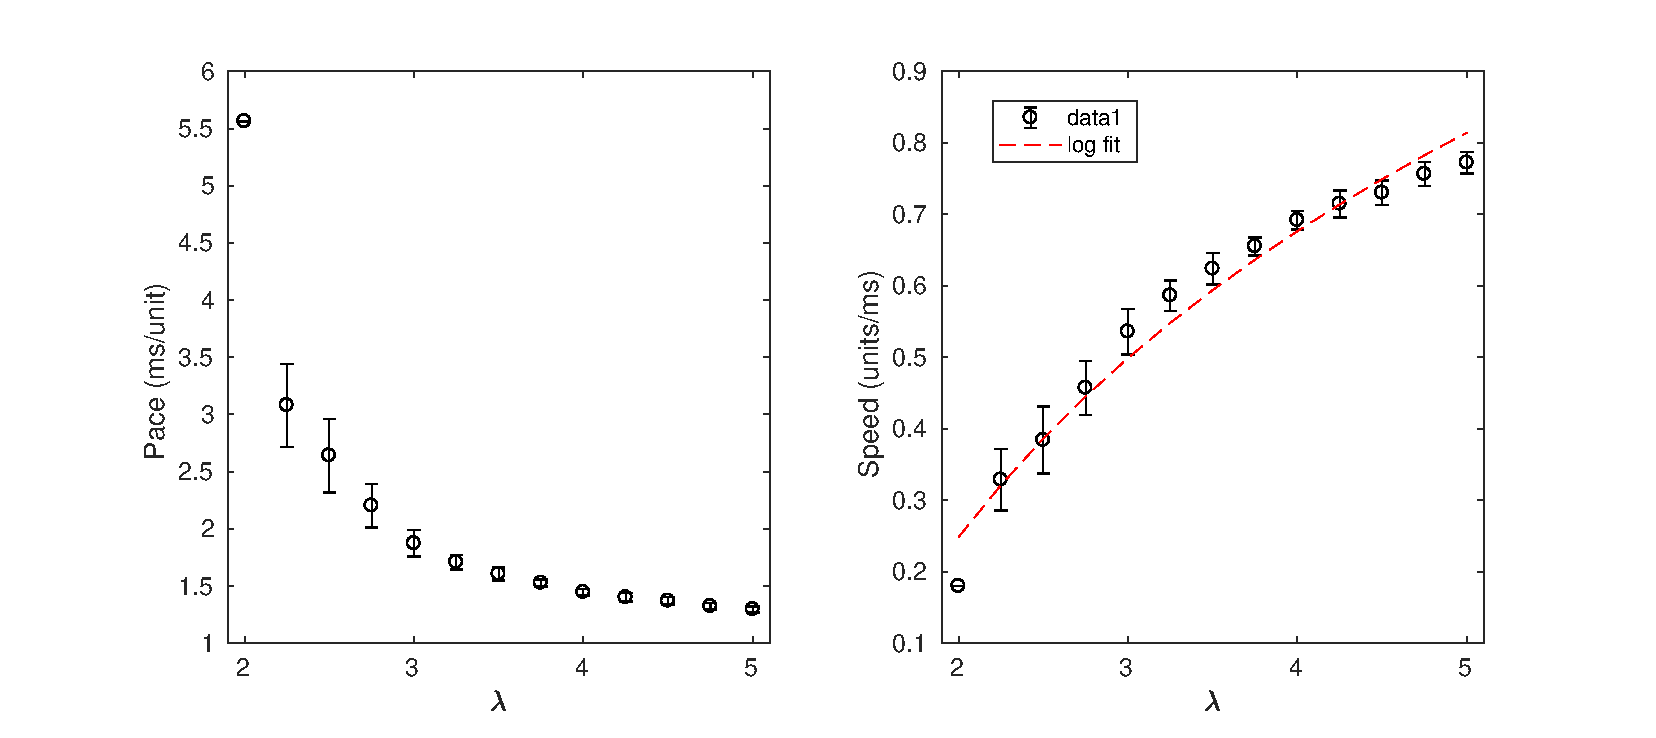
\includegraphics[width=\textwidth]{fig/WaveSpeed_Lambda}
\end{figure}

\FloatBarrier

Our SCE topology (namely, the X and Y dimensions) may influence the wave speed in several ways.
Increasing X and/or Y increases the total number of neurons, the total number of connections, and the average number of connections per neuron.
To test these, we construct columns with topology in XxY of $2x2, 2x3, 3x3, 3x4$ and $4x4$.
We also tested the $1x1$ topology but found that it did not support traveling waves (SI Figure 6).
For each topology we measure the pace and speed over $5$ randomly generated SCE (Figure \ref{fig:delay_topology}).
We see that increasing the X and/or Y dimensions of the SCE increases the speed, and the dependence looks qualitatively similar to increasing the connection strength via $K$ or the number of connections via $\lambda$.

\begin{figure}[!htb]
 \caption{ The pace (left, error bars $\pm 1 \sigma$) decreases, and the speed (right) increases, as the XxY extents of the SCE grow.}
 \label{fig:delay_topology}
 \centering
   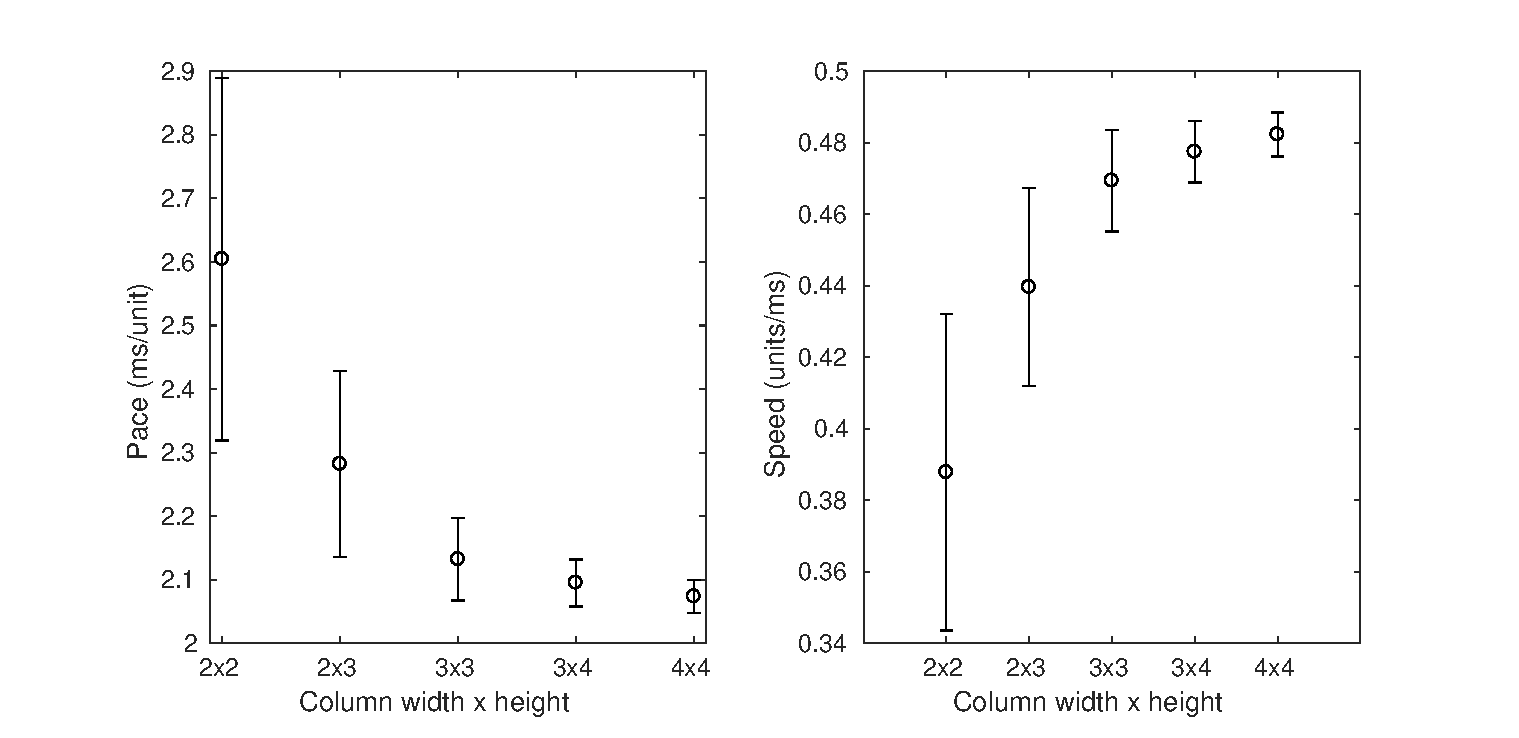
\includegraphics[width=\textwidth]{fig/WaveSpeed_Topology}
\end{figure}

To separate the effect of the increased connectivity from the effect of different topology (larger X or Y increases both the total number of neurons and changes the proportion of surface neurons) we scale the $C$ parameter in equation \ref{eq:connectivity} to maintain the same average number of connections per neuron (\textasciitilde{}7) across the topologies.
Results show that when separated from the increase in connectivity larger cross sections do not change the wave propagation speed (Figure \ref{fig:delay_topology_avgconn}).
Therefore the increase in speed with cross-section seen in Figure \ref{fig:delay_topology} is due entirely to the increasing number of connections per neuron.
Figure 5 in the SI shows additional analysis of SCE with larger cross sections. 

\begin{figure}[!htb]
 \caption{ Wave speed (error bars $1\sigma$) is constant as the topology changes as long as the average number of connections (~7 connections per neuron) is maintained. The largest topology is $13x13$ (169 neurons at base).}
 \label{fig:delay_topology_avgconn}
 \centering
   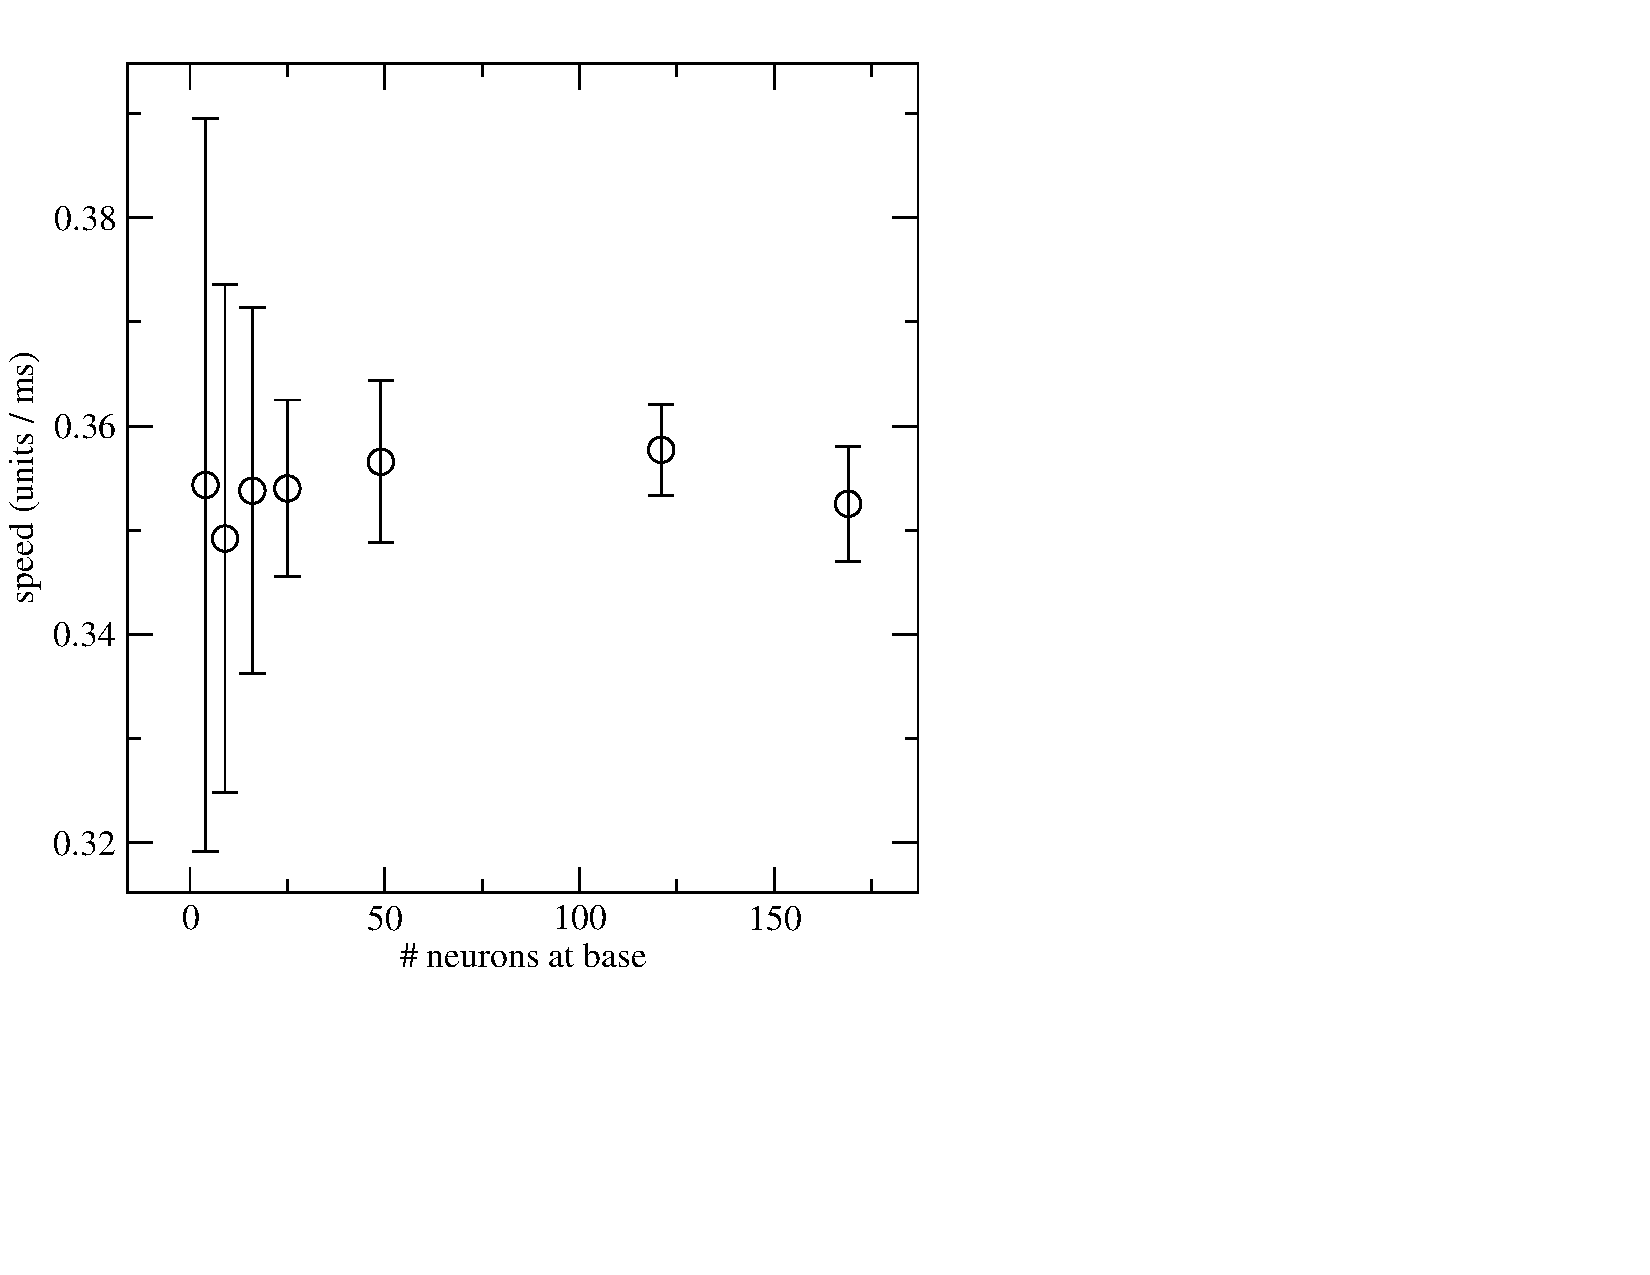
\includegraphics[width=\textwidth]{fig/speed_vs_thick_m}
\end{figure}

\FloatBarrier

It is interesting to compare the speeds obtained here with previous work.
We have placed our neurons on a unit grid and measured speed in units per millisecond.
By assuming that our unit grid is about $20~\mu m$ (Cruz et al., 2005) then our wave propagation speeds are in the range of $2-16~mm/s$.
This is generally slower than other computational results, but the mid to upper range is of the same order of magnitude as the experimental velocity of $50~mm/s$  reported in \citet{Golomb1997}.

\FloatBarrier

\section{Wave Initiation and Density} \label{sub:wave_initiation}
Traveling waves spawned by uniform background stimulation do not appear to originate at random places in the SCE.
Instead we observe that, for a given randomly generated SCE, waves tend to spawn from certain locations within the SCE.
This is most noticeable for SCEs with very dense local connectivity with $C=1.0$ in equation \ref{eq:connectivity}.
To quantify this observation we record the initiation sites of all traveling waves that were observed in an SCE under uniform background stimulus (Figure \ref{fig:wave_initiation_sites}).
We then measure the fraction of wave initiation events (FIE) per unit length of the SCE.

\begin{figure}[!htb]
 \caption{Left: The time and place of origin of every traveling wave produced during a simulation. Right: The FIE clearly shows that traveling waves are likely to start in some regions, and unlikely to start in others.}
 \label{fig:wave_initiation_sites}
 \centering
   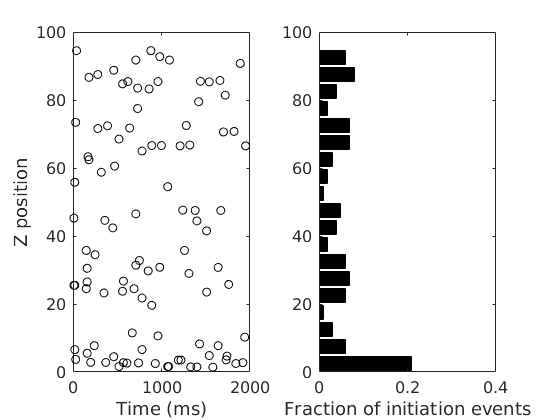
\includegraphics[width=\textwidth]{fig/InitiationSites_100sims}
\end{figure}

A separate observation is that only some of the neurons in the SCE will fire when a wave passes their location.
We observe that a single traveling wave initiated by a step stimulus can have regions of higher or lower total firing activity which we quantify by measuring the fractional number of firing events (FFE) per unit length of the SCE.
An example measurement of the firing activity in a single traveling wave is shown in Figure \ref{fig:wave_density}.
\begin{figure}[!htb]
 \caption{Density of firing events in a traveling wave initiated from a step stimulus. Left: Raster plot of the spike-emission times from a single traveling wave. Right: The FFE shows that some regions of the SCE exhibit more firing activity.}
 \label{fig:wave_density}
 \centering
   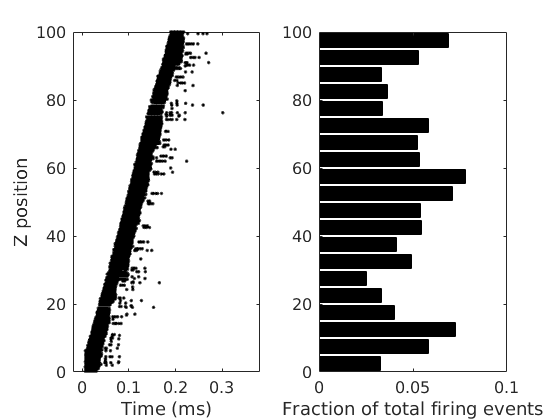
\includegraphics[width=\textwidth]{fig/ImpulseWaveDensity}
\end{figure}

By combining these two experiments we observe that the results from the FIE and the FFE appear anti-correlated. 
In Figure \ref{fig:fie_ffe_plots} we see multiple FIE and FFE plots from the same SCE placed side-by-side.
There is a visual anti-correlation between the FIE and FFE for each SCE although it is not conclusive from these plots.
\begin{figure}[!htb]
 \caption{FIE and FFE for nine example columns. } 
 \begin{tabular}{ccc}
     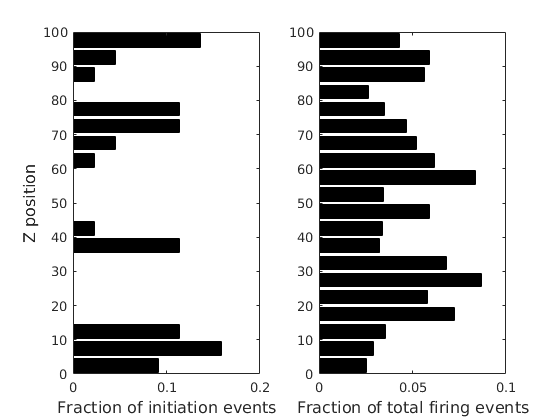
\includegraphics[width=0.3\textwidth]{fig/ccf/ccf1} & 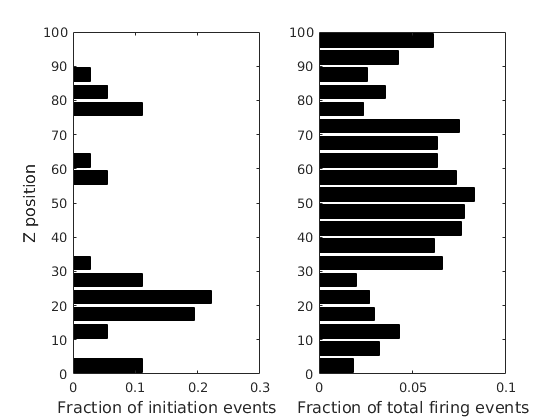
\includegraphics[width=0.3\textwidth]{fig/ccf/ccf2} & 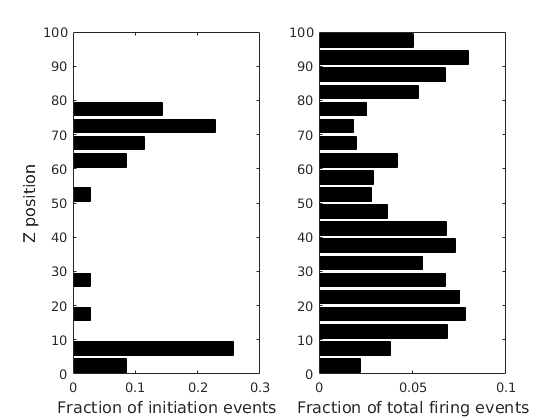
\includegraphics[width=0.3\textwidth]{fig/ccf/ccf3} \\
     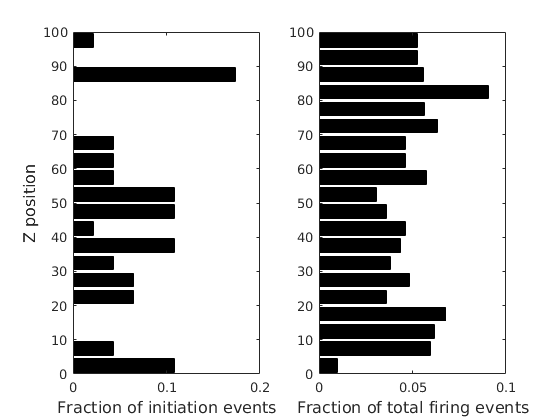
\includegraphics[width=0.3\textwidth]{fig/ccf/ccf4} & 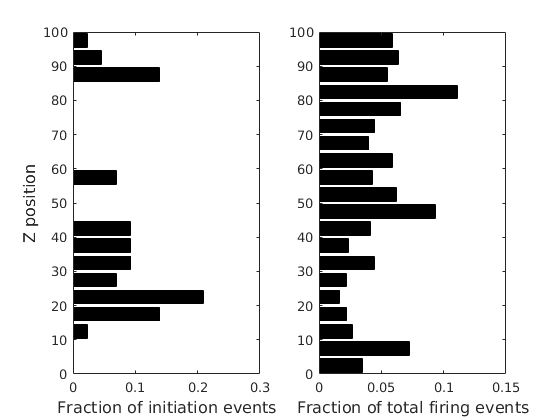
\includegraphics[width=0.3\textwidth]{fig/ccf/ccf5} & 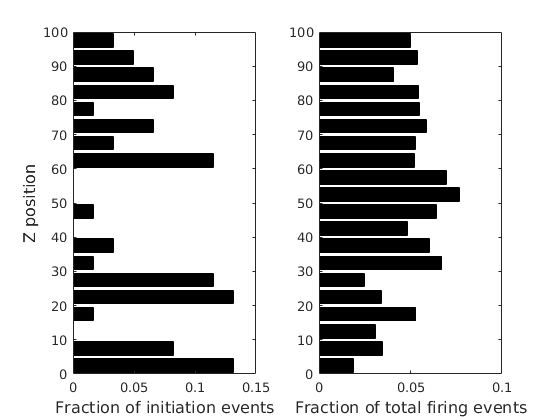
\includegraphics[width=0.3\textwidth]{fig/ccf/ccf6} \\
     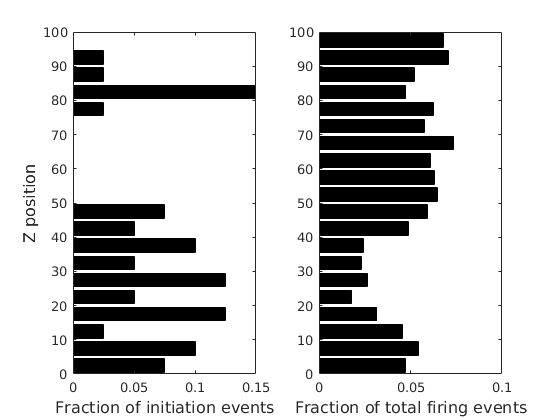
\includegraphics[width=0.3\textwidth]{fig/ccf/ccf7} & 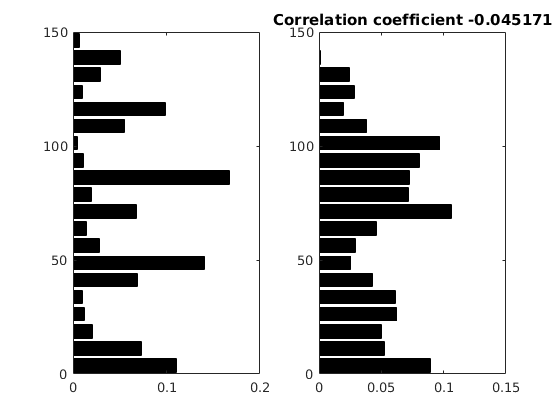
\includegraphics[width=0.3\textwidth]{fig/ccf/ccf8} & 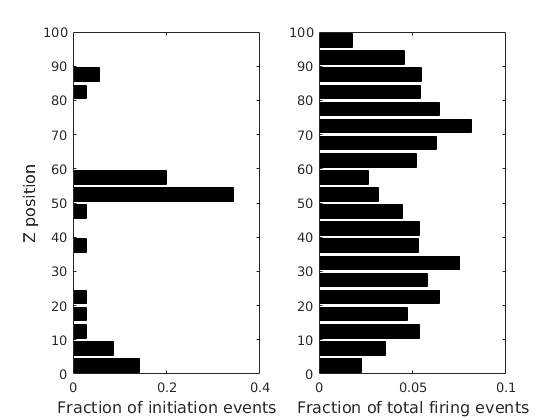
\includegraphics[width=0.3\textwidth]{fig/ccf/ccf9} 
 \end{tabular}
 \label{fig:fie_ffe_plots}
\end{figure}

\FloatBarrier

To test that this observation is generally true we create 100 SCEs, apply first uniform background stimulus and then step stimulus to each SCE, and measure the correlation between the FIE and FFE (Figure \ref{fig:InitiationCorrelation}).
The correlation coefficient is estimated from the two histograms using MATLAB 'corrcoef'.  
Although there is substantial variation between SCEs we measure a consistently negative correlation coefficient (mean $-0.26$, standard deviation $0.18$) between FIE and FFE results.
A one-sided t-test at the $1\%$ confidence level rejects the null hypothesis that the mean of the correlation coefficient is $0$ or greater.
\begin{figure}[!htb]
 \centering
 \caption{ A) Correlation between FIE and FFE across 100 trials. B) Distribution of the correlation coefficient. Each trial is a new SCE with random neuron and connectivity parameters. }
 \label{fig:InitiationCorrelation}
 \begin{tabular}{c}
     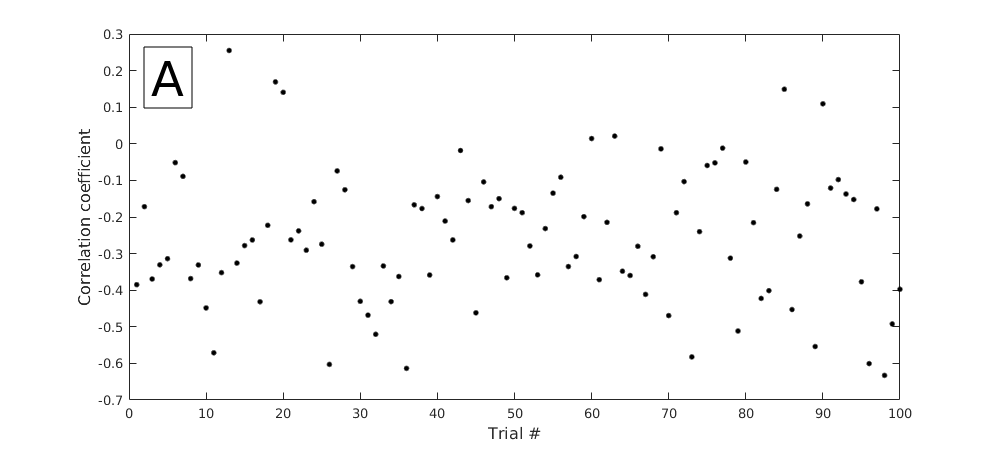
\includegraphics[width=\textwidth]{fig/InitiationCorrelation} \\ 
     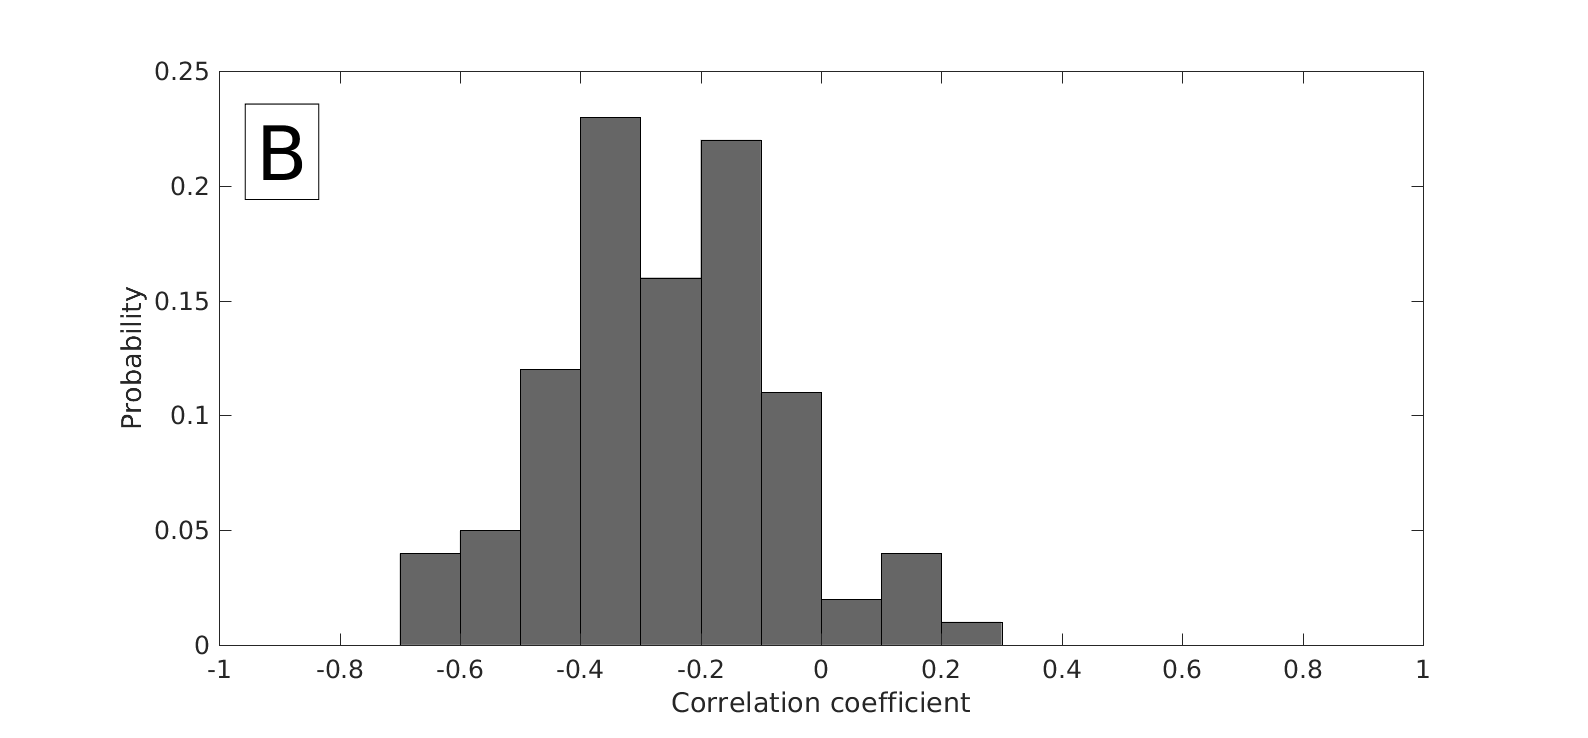
\includegraphics[width=\textwidth]{fig/InitiationCorrelationPDF} 
 \end{tabular}
\end{figure}

We hypothesize that these preferential wave initiation sites are created by neurons with low firing thresholds that are easy to excite.
In the Izhikevich model, inhibitory neurons can have a lower firing threshold than excitatory neurons, modeling the behavior of real inhibitory neurons in the cortex\citet{gibson2009}\citet{hayut2011}.
As we can see from figure \ref{fig:delay_neurondynamics}  the $b$ parameter in the Izhikevich model sets the firing threshold of the individual neurons.
Neurons with higher $b$ parameter are easier to excite and therefore more likely to fire.
Per Table \ref{tab:izzy_params} excitatory neurons all have a $b$ parameter of $0.2$, while inhibitory neurons have $b$ parameters in the range $0.2-0.25$.
This indicates the preferential wave initiation sites could be due to low-threshold spiking (LTS) inhibitory neurons \citet{izhikevich2003}.
It may seem counter-intuitive that firing activity from an \underline{inhibitory} neuron would generate traveling waves.
In fact, postinhibitory rebound spiking is observed in both cortical neurons \citet{ascoli2010} and the Izhikevich model of neuron dynamics,  and was studied in the context of spindle waves in the thalamus in \citet{Golomb1996}.
The LTS hypothesis also explains the reduced wave density at these sites.
As a traveling wave passes through the region, because of their increased activity these same inhibitory neurons suppress the surrounding neurons resulting in fewer local firing events.

A comparative computational experiment shows that low-threshold spiking inhibitory neurons can indeed generate traveling waves under background stimulus.
We first create an SCE with entirely excitatory neurons.
We then create an identical SCE except for a single LTS inhibitory neuron at $Z=50$.
The $b$ parameter of the LTS inhibitory neuron is set to $0.25$, corresponding to the lowest firing threshold used in our model.
These two SCEs are stimulated with the same uniform background stimulus. 
Figure \ref{fig:lts_inhibit} clearly shows that adding the single LTS neuron results in traveling waves emanating from $Z=50$. 
\begin{figure}[!htb]
 \caption{Simulation with a single LTS inhibitory neuron at $Z=50$. Left: an SCE with entirely excitatory neurons shows traveling waves emerging from various locations. Right: adding a single LTS neuron at $Z=50$ results in consistent wave generation from that location. }
 \label{fig:lts_inhibit}
 \centering
   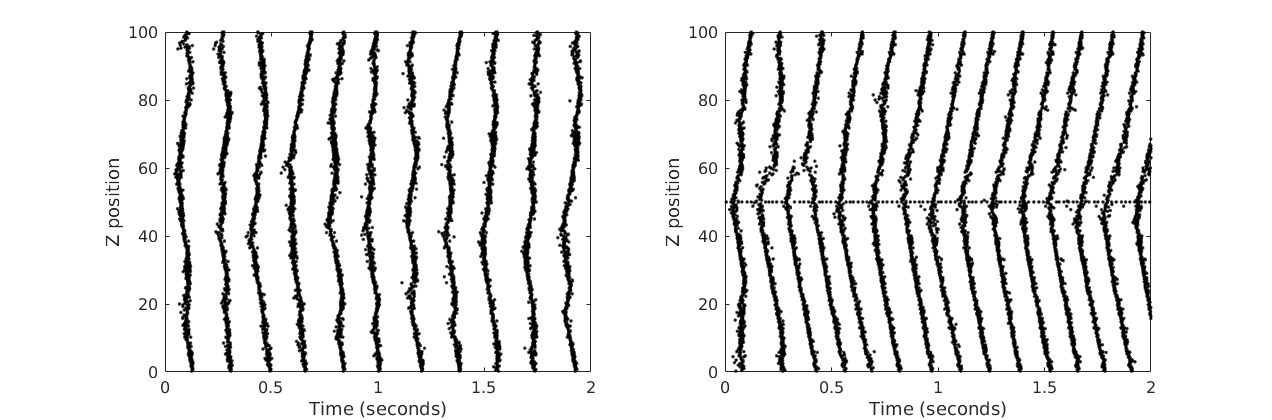
\includegraphics[width=\textwidth]{fig/SingleLTSInhibit}
\end{figure}

\FloatBarrier

\subsection{Wave patterns in fully connected networks} \label{sub:delay}
Our investigation has been concerned with traveling waves of activations that spread through locally connected networks.
We now examine whether traveling wave patterns can also be observed in fully connected networks.
We show that this is possible provided we consider the action potential propagation delay proportional to the distance between neurons, as used in all the simulations above.
We simulate an SCE with complete connectivity corresponding to $\lambda \rightarrow \infty$: all neurons are connected with probability 1 to all other neurons.
This is analogous to the original Izhikevich simulation \citet{izhikevich2003} that demonstrated synchronized firing in a completely connected neural field with random background stimulus.
We first simulate the SCE with a fixed action potential propagation delay of $1.7~ms$ \citet{Markram1997}  regardless of inter-neuron distance.
The result is highly synchronized simultaneous firing among all neurons in the SCE.
 
With distance-dependent propagation delays and fast spike propagation ($\kappa=0.1$) we observe similar synchronized firing.
We then increase $\kappa$ and observe the emergence of traveling wave patterns (Figure \ref{fig:delay_waves}). 
This demonstrates that one dimensional traveling waves can emerge from fully-connected networks if the propagation delay is proportional to the inter-neuron distance and the spike propagation time is above a critical value.
\begin{figure}[!htb]
 \caption{With global connectivity and action potential propagation delay fixed at $1.7~ms$ , the entire structure shows synchronized firing events.
          With distance-dependent propagation we also observe synchronized firing at $\kappa=0.1$.
          As $\kappa$ increases traveling waves emerge ($\kappa=0.5, 1.0$) .}
 \centering
   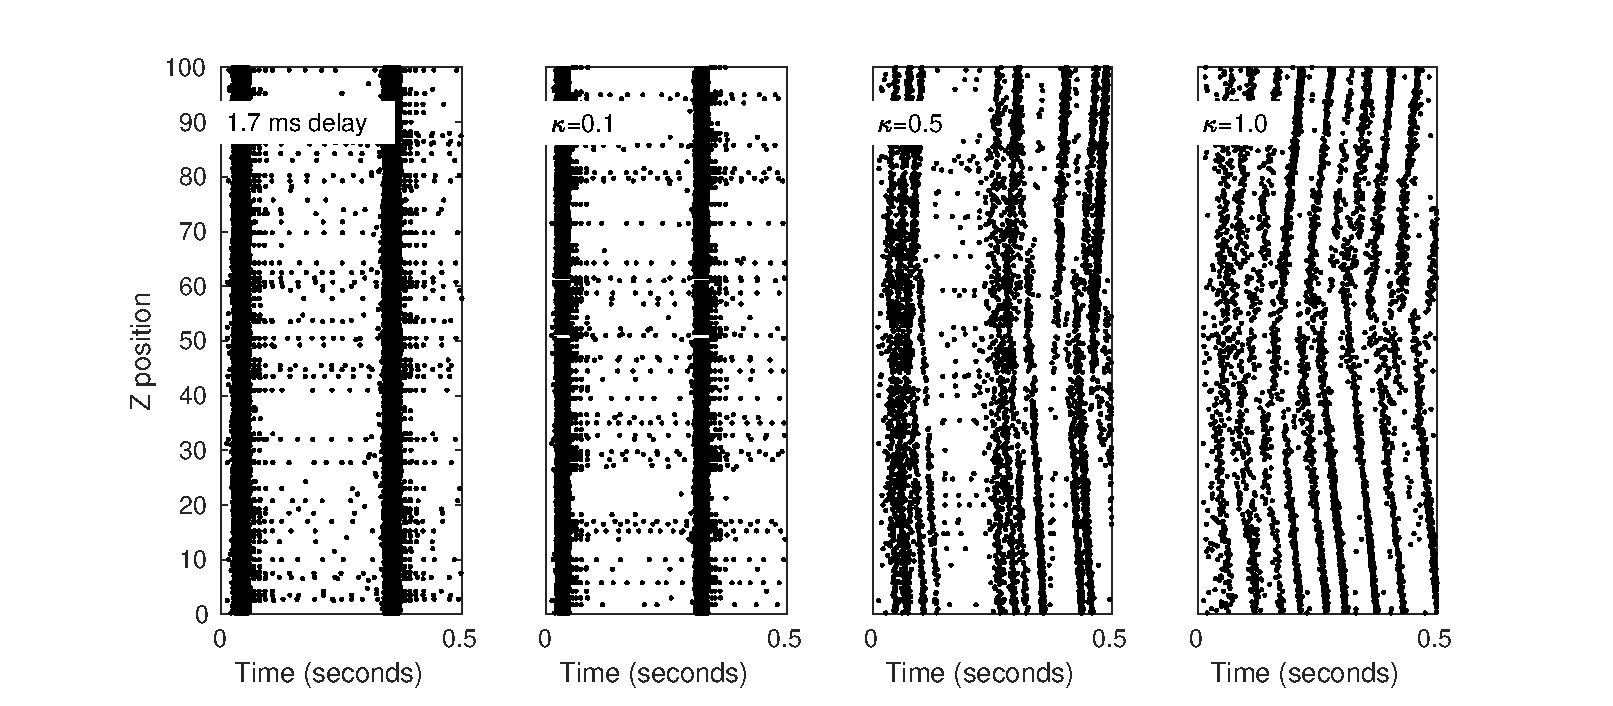
\includegraphics[width=\textwidth]{fig/DelayWaves}  
 \label{fig:delay_waves}
\end{figure}

The present case is similar to previous work that considered coupled oscillators  (\citet{ermentrout2001}, Figure 1) that proposed several models for traveling waves in the cortex.
The one most relevant to traveling waves in our fully-connected networks is a driving source at a spatial location that produces traveling wave patterns due to the propagation delay of action potentials.
This is a fundamentally different type of traveling wave than a chain of spike events that spreads to neighboring neurons due to local connectivity.

\endinput
%%
%% End of file `example-1.tex'.
